% This document is compiled using pdfLaTeX
% You can switch XeLaTeX/pdfLaTeX/LaTeX/LuaLaTeX in Settings

\documentclass{article}
\PassOptionsToPackage{quiet}{fontspec}
\usepackage{amsmath, amsthm, amssymb, amsfonts}
\usepackage{thmtools}
\usepackage{graphicx}
\usepackage{setspace}
\usepackage{geometry}
\usepackage{float}
\usepackage{hyperref}
\usepackage[UTF8]{ctex}
\usepackage{framed}
\usepackage[dvipsnames]{xcolor}
\usepackage{tcolorbox}

\colorlet{LightGray}{White!90!Periwinkle}
\colorlet{LightOrange}{Orange!15}
\colorlet{LightGreen}{Green!15}

\newcommand{\HRule}[1]{\rule{\linewidth}{#1}}


% definition 
\declaretheoremstyle[name=Definition,]{thmsty}
\declaretheorem[style=thmsty,numberwithin=section]{definition}
\tcolorboxenvironment{definition}{colback=White}

% theorem
\declaretheoremstyle[name=Theorem,]{thmsty}
\declaretheorem[style=thmsty,numberwithin=section]{theorem}
\tcolorboxenvironment{theorem}{colback=White}

% lemma
\declaretheoremstyle[name=Lemma,]{thmsty}
\declaretheorem[style=thmsty,numberwithin=section]{lemma}
\tcolorboxenvironment{lemma}{colback=White}
%proposition 
\declaretheoremstyle[name=Proposition,]{prosty}
\declaretheorem[style=prosty,numberlike=theorem]{proposition}
\tcolorboxenvironment{proposition}{colback=White}

% remark
\declaretheoremstyle[name=Remark,]{thmsty}
\declaretheorem[style=thmsty,numberwithin=section]{remark}
% \tcolorboxenvironment{remark}{colback=White}


% % proof
% \declaretheoremstyle[name=Proof,]{prosty}
% \declaretheorem[style=prosty,numberlike=theorem]{proof}




\setstretch{1.2}
\geometry{
    textheight=9in,
    textwidth=5.5in,
    top=1in,
    headheight=12pt,
    headsep=25pt,
    footskip=30pt
}

\title{平面几何-三角法}
\author{}
\date{}




\begin{document}

\maketitle

\section{三角法常用结论}
\begin{theorem}[正弦定理]
    任意$\triangle ABC$中,各边和它所对角的正弦值之比相等,且等于外接圆直径长,即
    $$
\frac{AB}{\sin C}=\frac{BC}{\sin A}=\frac{CA}{\sin B}.
    $$
\end{theorem}

\begin{theorem}[分角线定理]
    $\triangle ABC$中,D为BC所在直线上一点,则有
    $$
    \frac{BD}{DC}  = \frac{AB}{AC}\cdot \frac{\sin\angle DAB}{\sin\angle DAC}.
    $$
    
    注意AD为中线或角平分线的特殊情况。
\end{theorem}

\begin{figure}[htbp]
    \centering
    % \hfill
    \begin{minipage}[t]{0.45\textwidth}
    \centering
    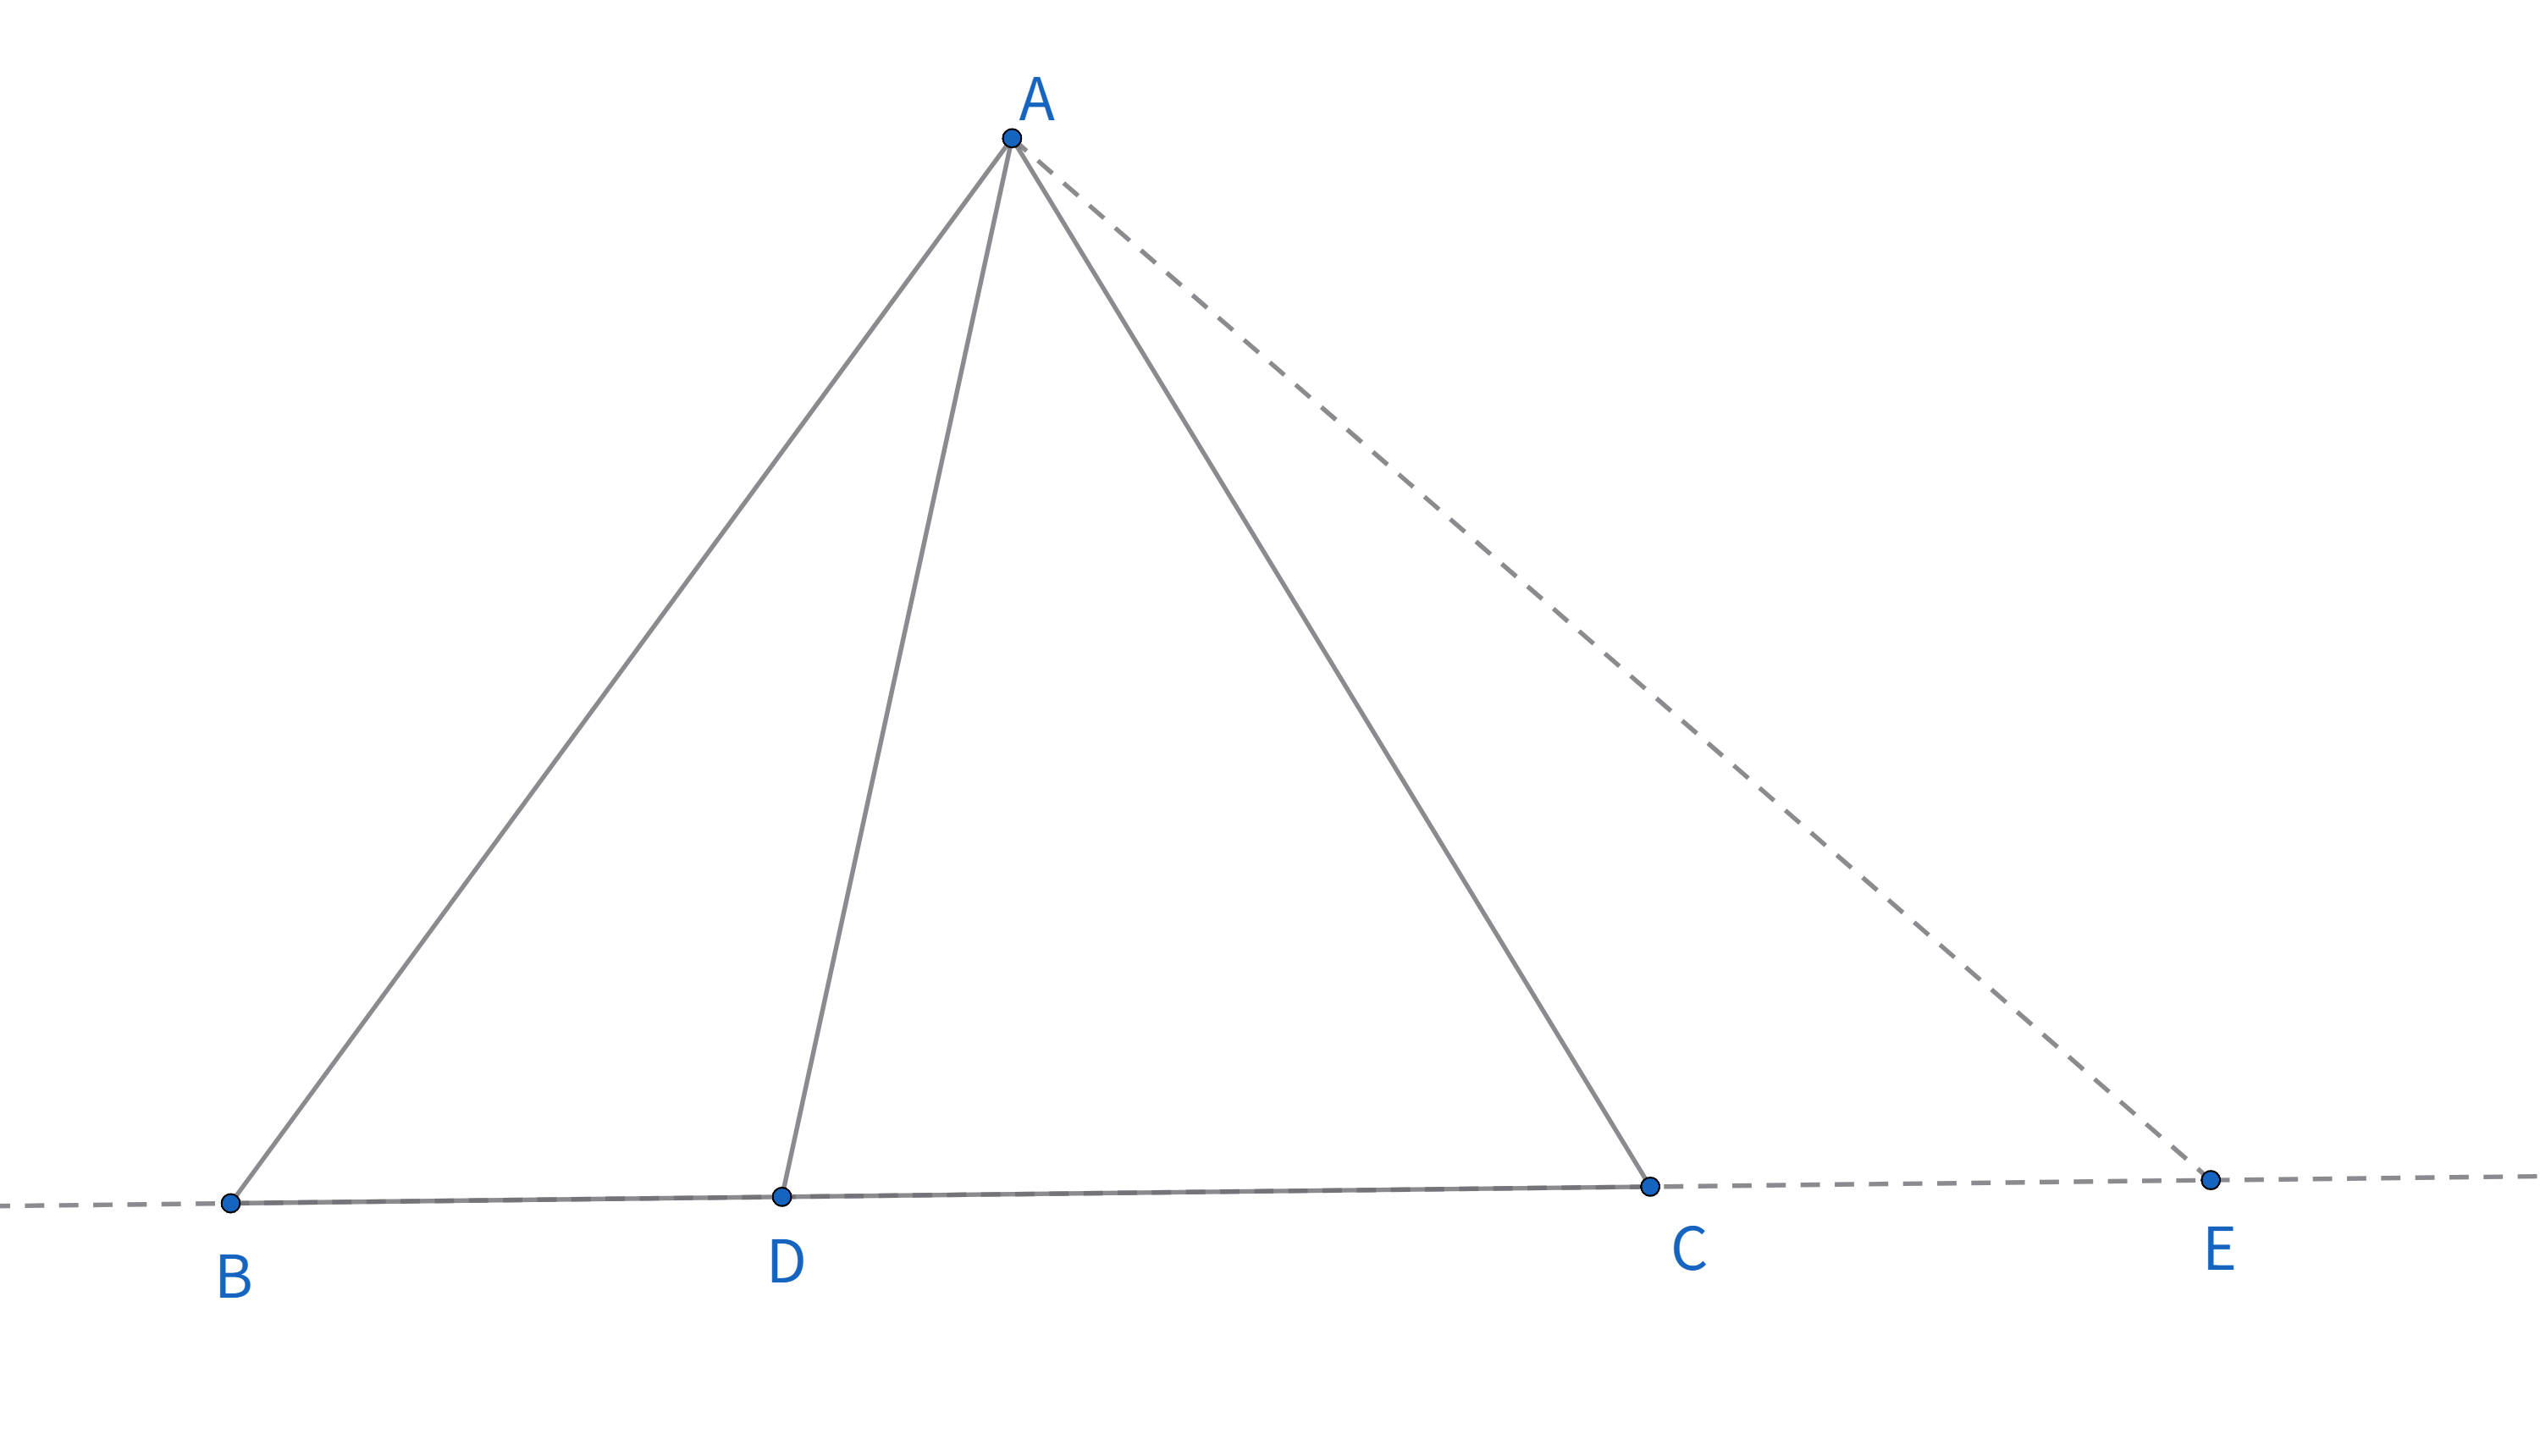
\includegraphics[width=0.8\linewidth]{figures/分角线定理.png}
    \end{minipage}
    % \hfill
    \begin{minipage}[t]{0.45\textwidth}
    \centering
    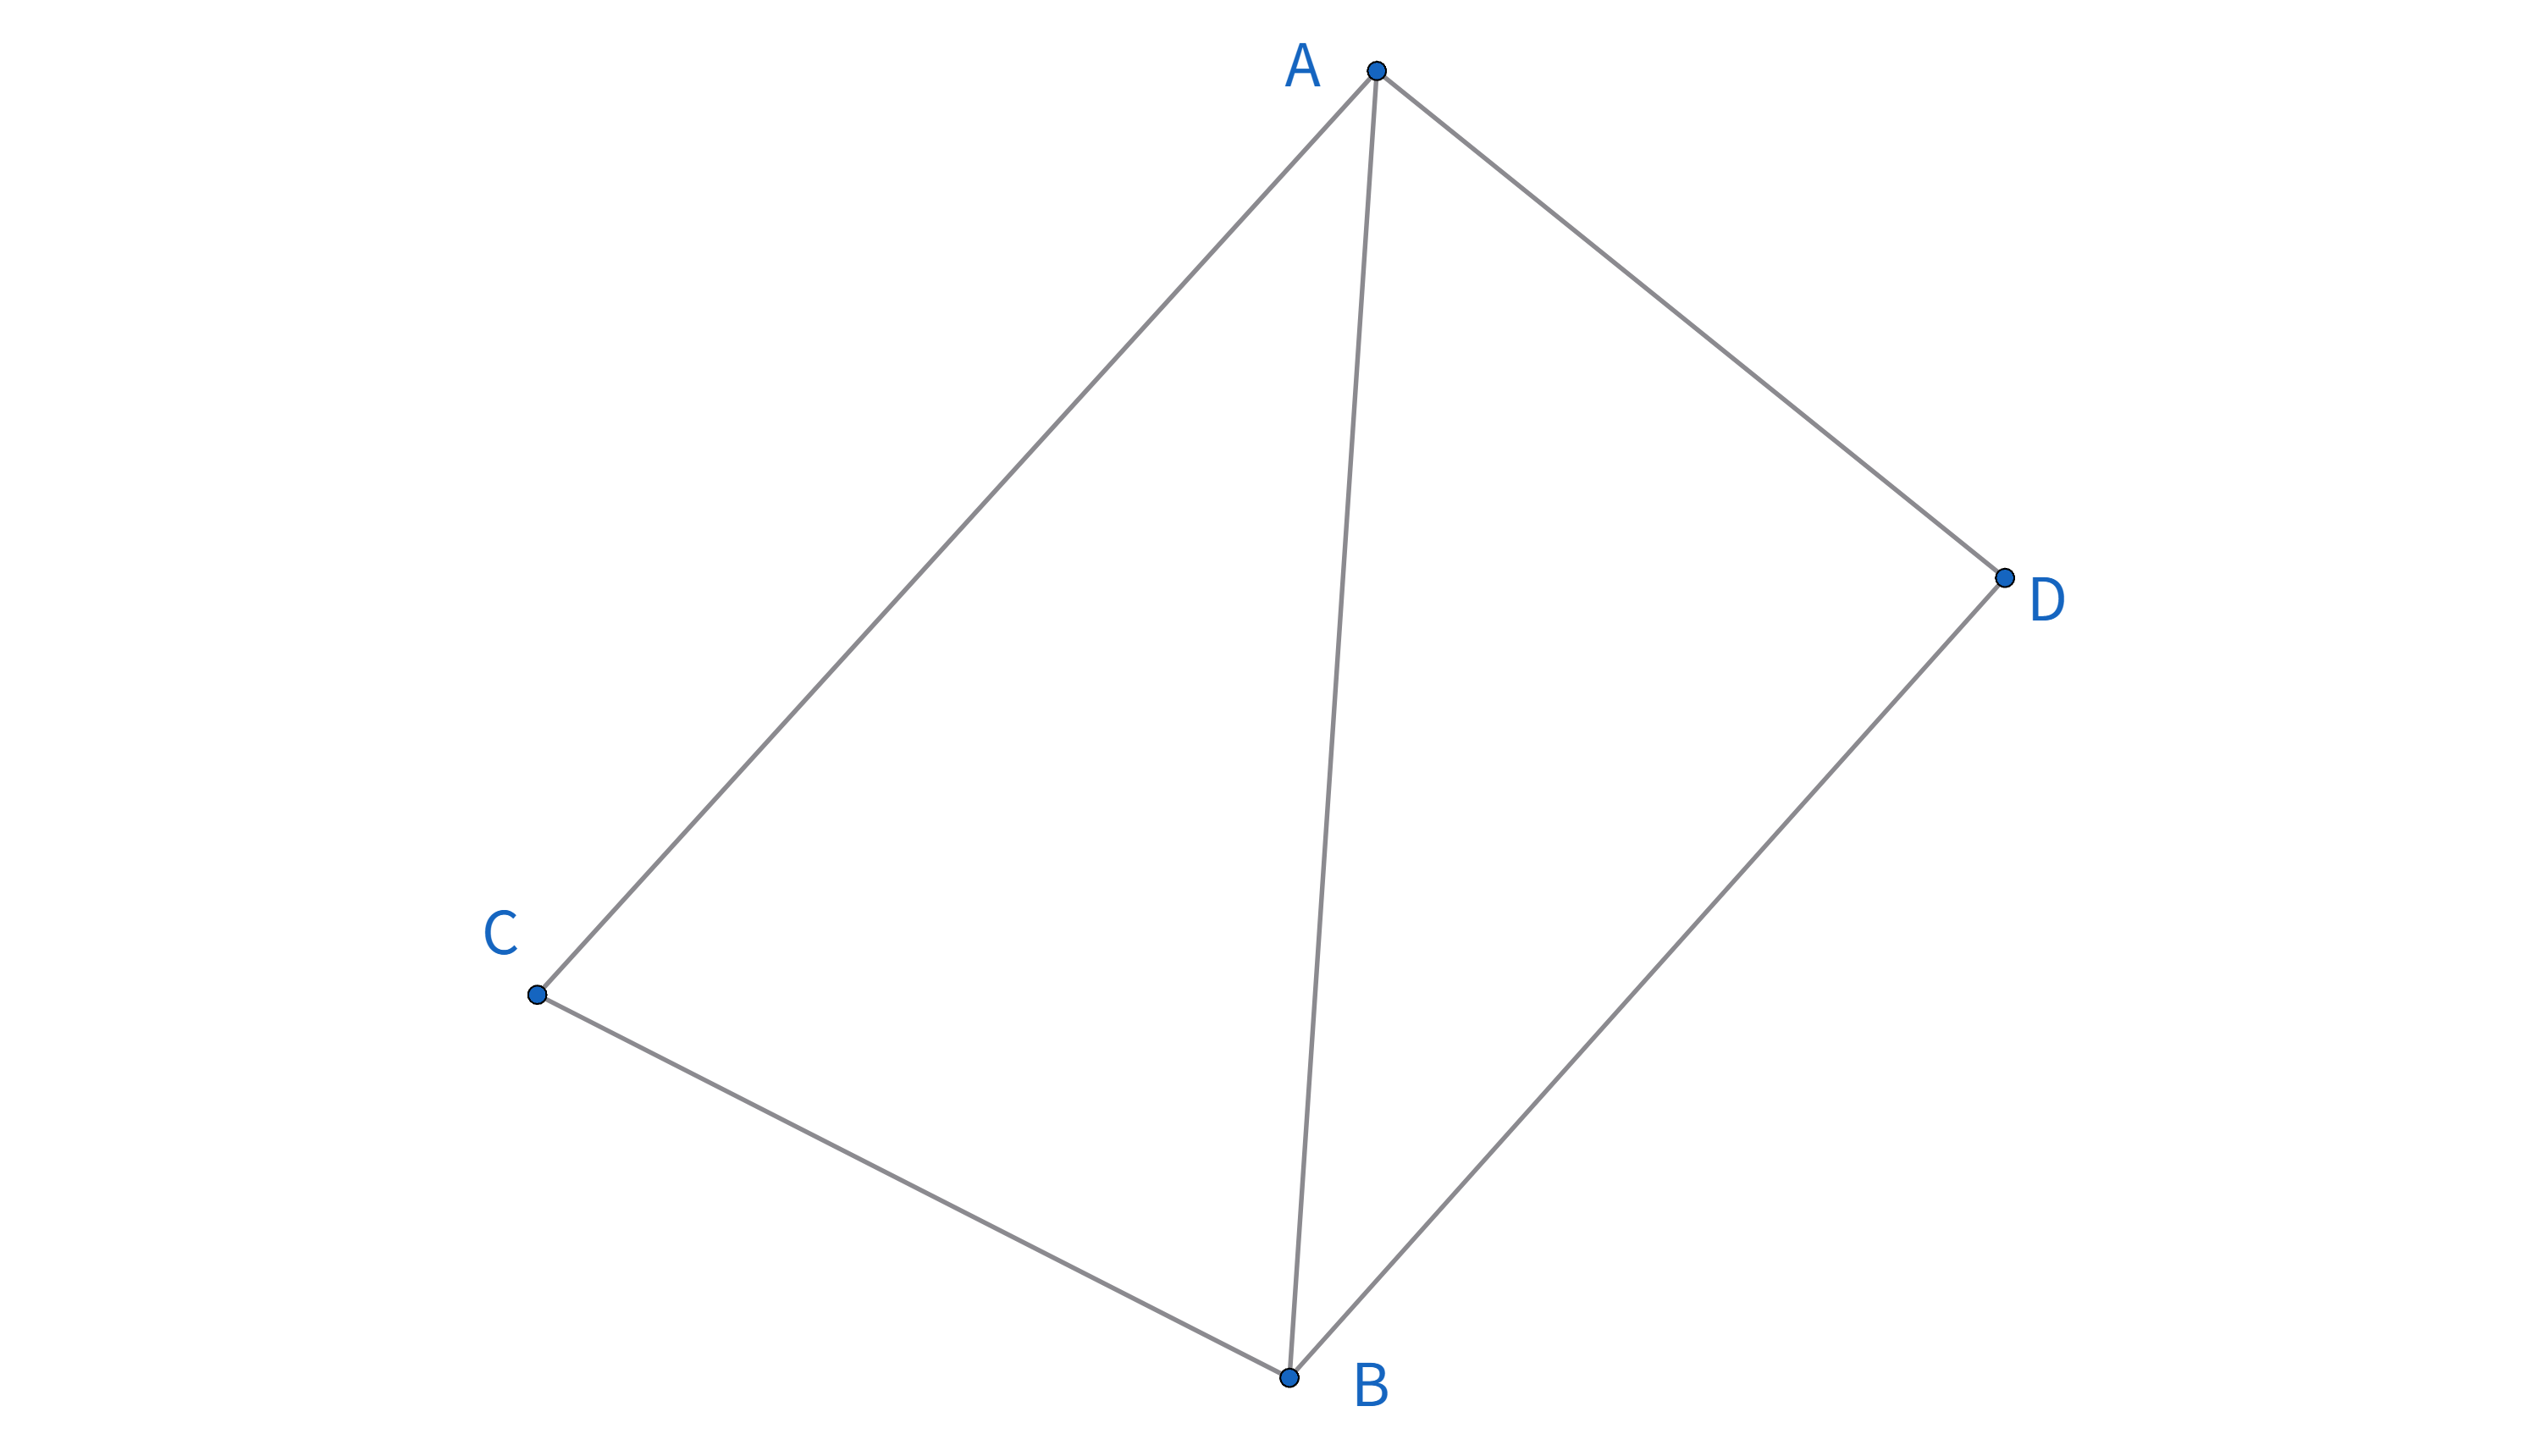
\includegraphics[width=0.8\linewidth]{figures/共边三角形.png}
    \end{minipage}
\end{figure}


\begin{proposition}
    设$\triangle ABC$与$\triangle ABD$共用AB边,则下列等式成立:
    $$
    \frac{\sin \angle BAC}{\sin \angle BAD} = \frac{BC}{BD} \cdot \frac{\sin\angle ACB}{\sin\angle ADB}.
    $$
\end{proposition}



\begin{proposition}
    给定$0<\alpha_1,\alpha_2,\beta_1,\beta_1<180^\circ$, 设$\alpha_1+\beta_1 = \alpha_2+\beta_2 <180^\circ$, 若
    $$
    \frac{\sin \alpha_1}{\sin \beta_1}=\frac{\sin \alpha_2}{\sin\beta_2},
    $$
    则有$\alpha_1 = \alpha_2, \beta_1=\beta_2.$
\end{proposition}


%-------------------------------------------------------------
\newpage 
\section{例题}
\subsection{Ex1}
给定$\triangle ABC$,内切圆与三边切点分别是D、E、F,过D作BC垂线交EF于点G,M为BC中点。证明:A、G、M三点共线。
\begin{figure}[htbp]
    \centering
    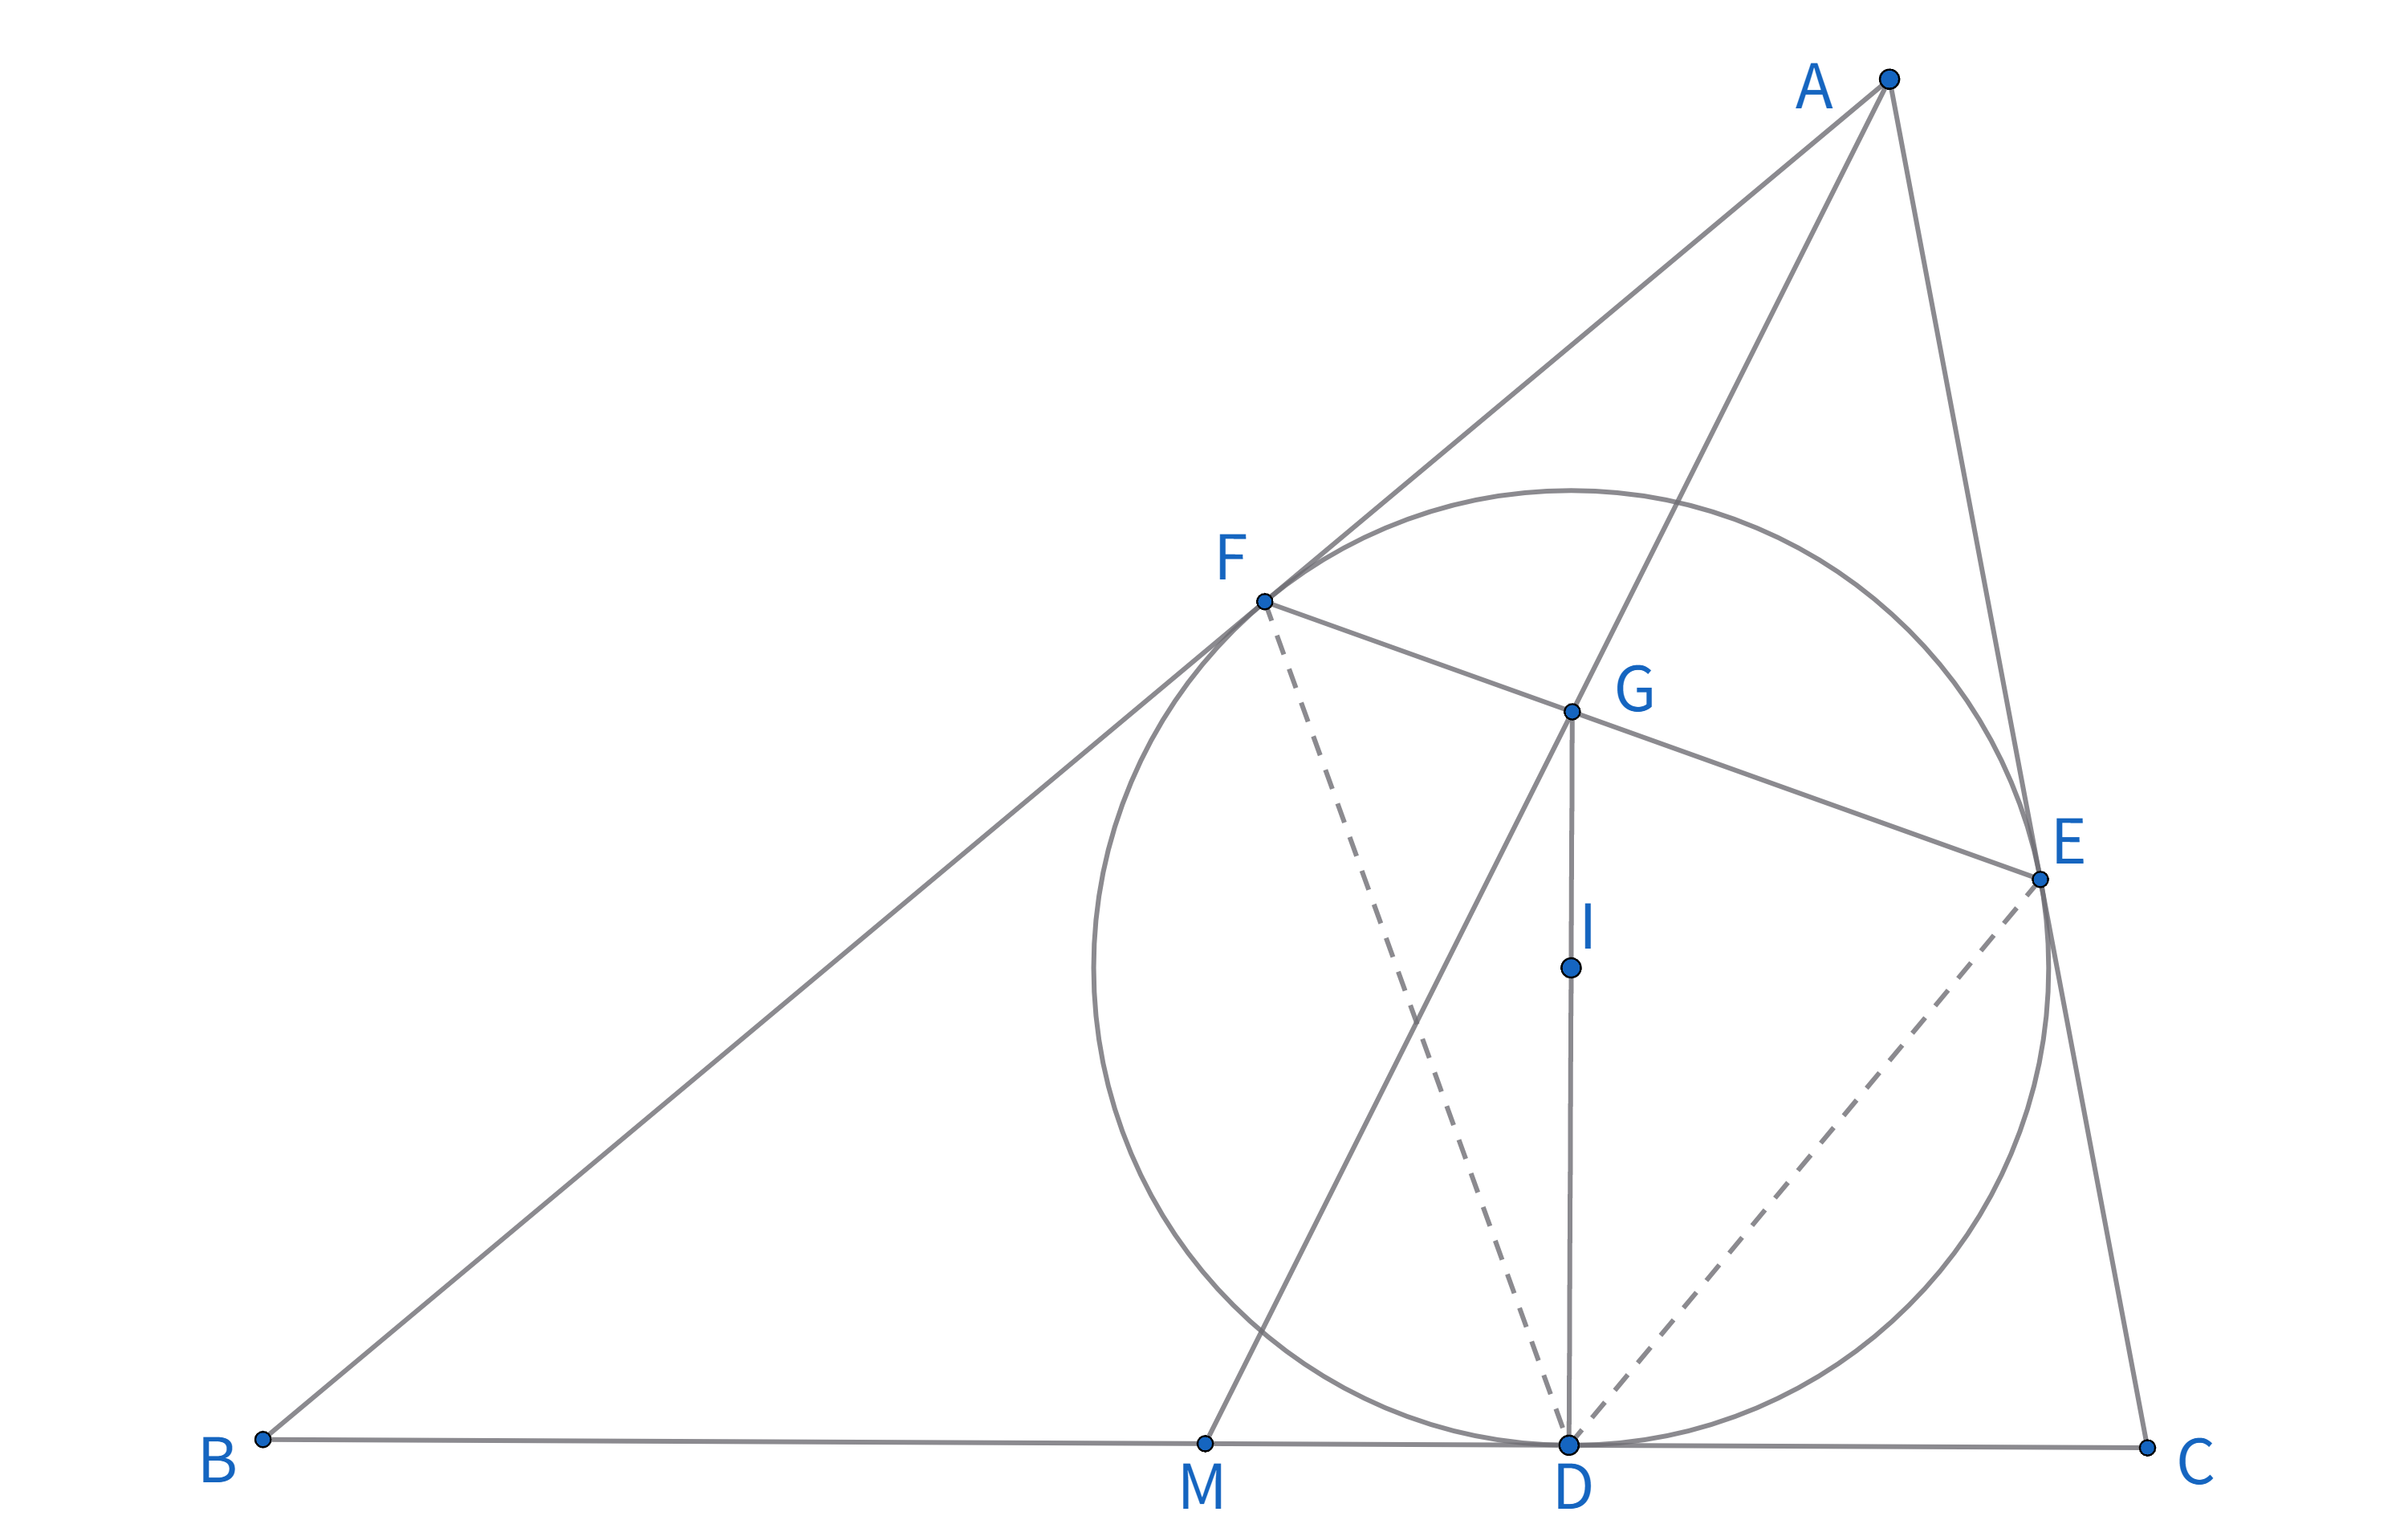
\includegraphics[width=0.8\linewidth]{figures/Ex1.png}
\end{figure}


\subsection{Ex2}
锐角$\triangle ABC$中,O为外接圆圆心,AH为BC边上高线,延长AO交BC于D,$\angle ADB, \angle ADC$内角平分线分别交AB、AC于E、F,证明:∠EHF=90°.
\begin{figure}[htbp]
    \centering
    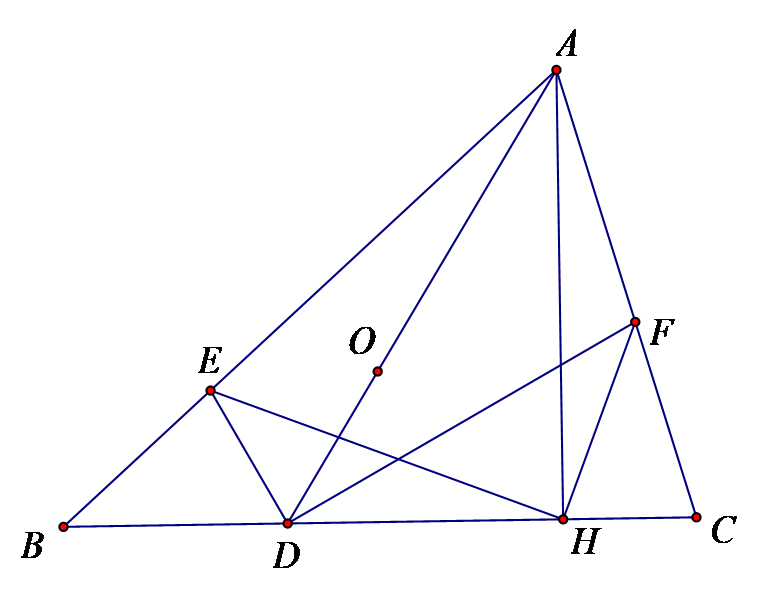
\includegraphics[width=0.8\linewidth]{figures/Ex2.png}
\end{figure}

%-------------------------------------------------------------
\newpage 
\subsection{Ex3}
给定平行四边形ABCD,DF、CE为$\triangle OCD$的两条高,过O做AD垂直线交BA延长线于G。证明:G、E、F共线。
\begin{figure}[htbp]
    \centering
    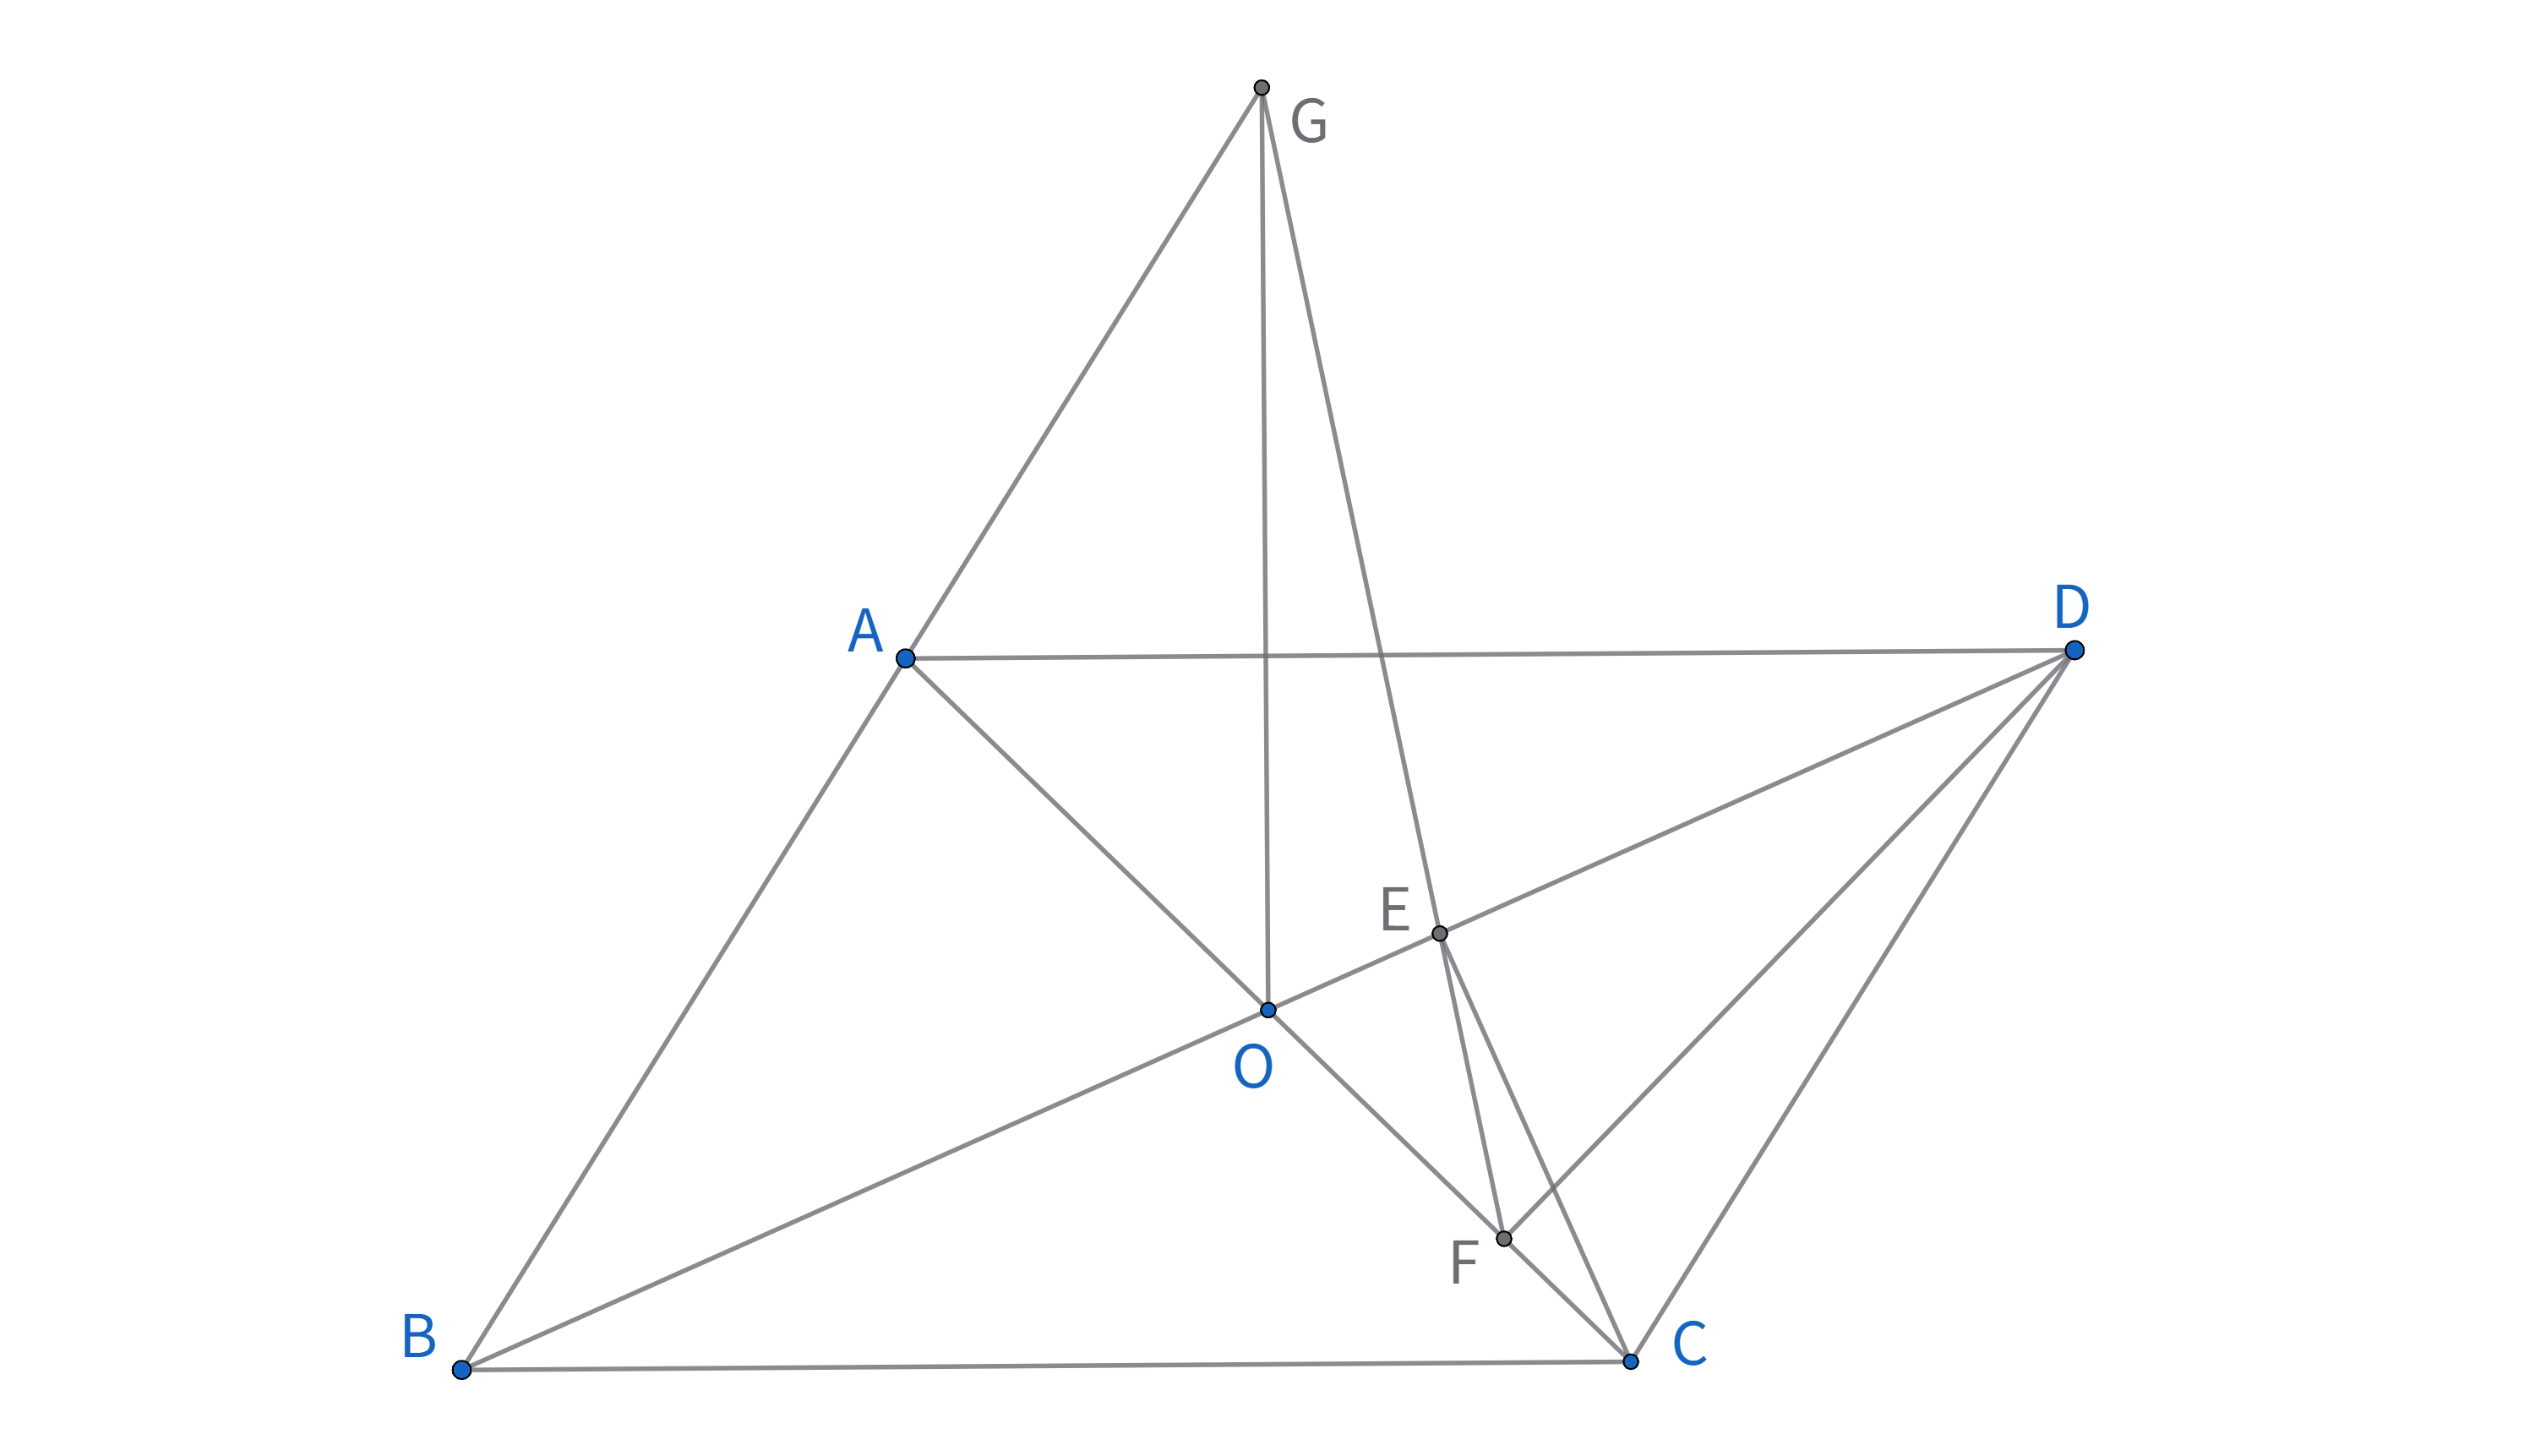
\includegraphics[width=0.9\linewidth]{figures/Ex3.png}
\end{figure}

\section{练习题}
\subsection{Q1}
设ABCD四点共圆,四边形ABDE为平行四边形。AC与BD交于点S,射线AB与DC交于点F。
证明:$\angle AFS=\angle ECD.$
\begin{figure}[htbp]
    \centering
    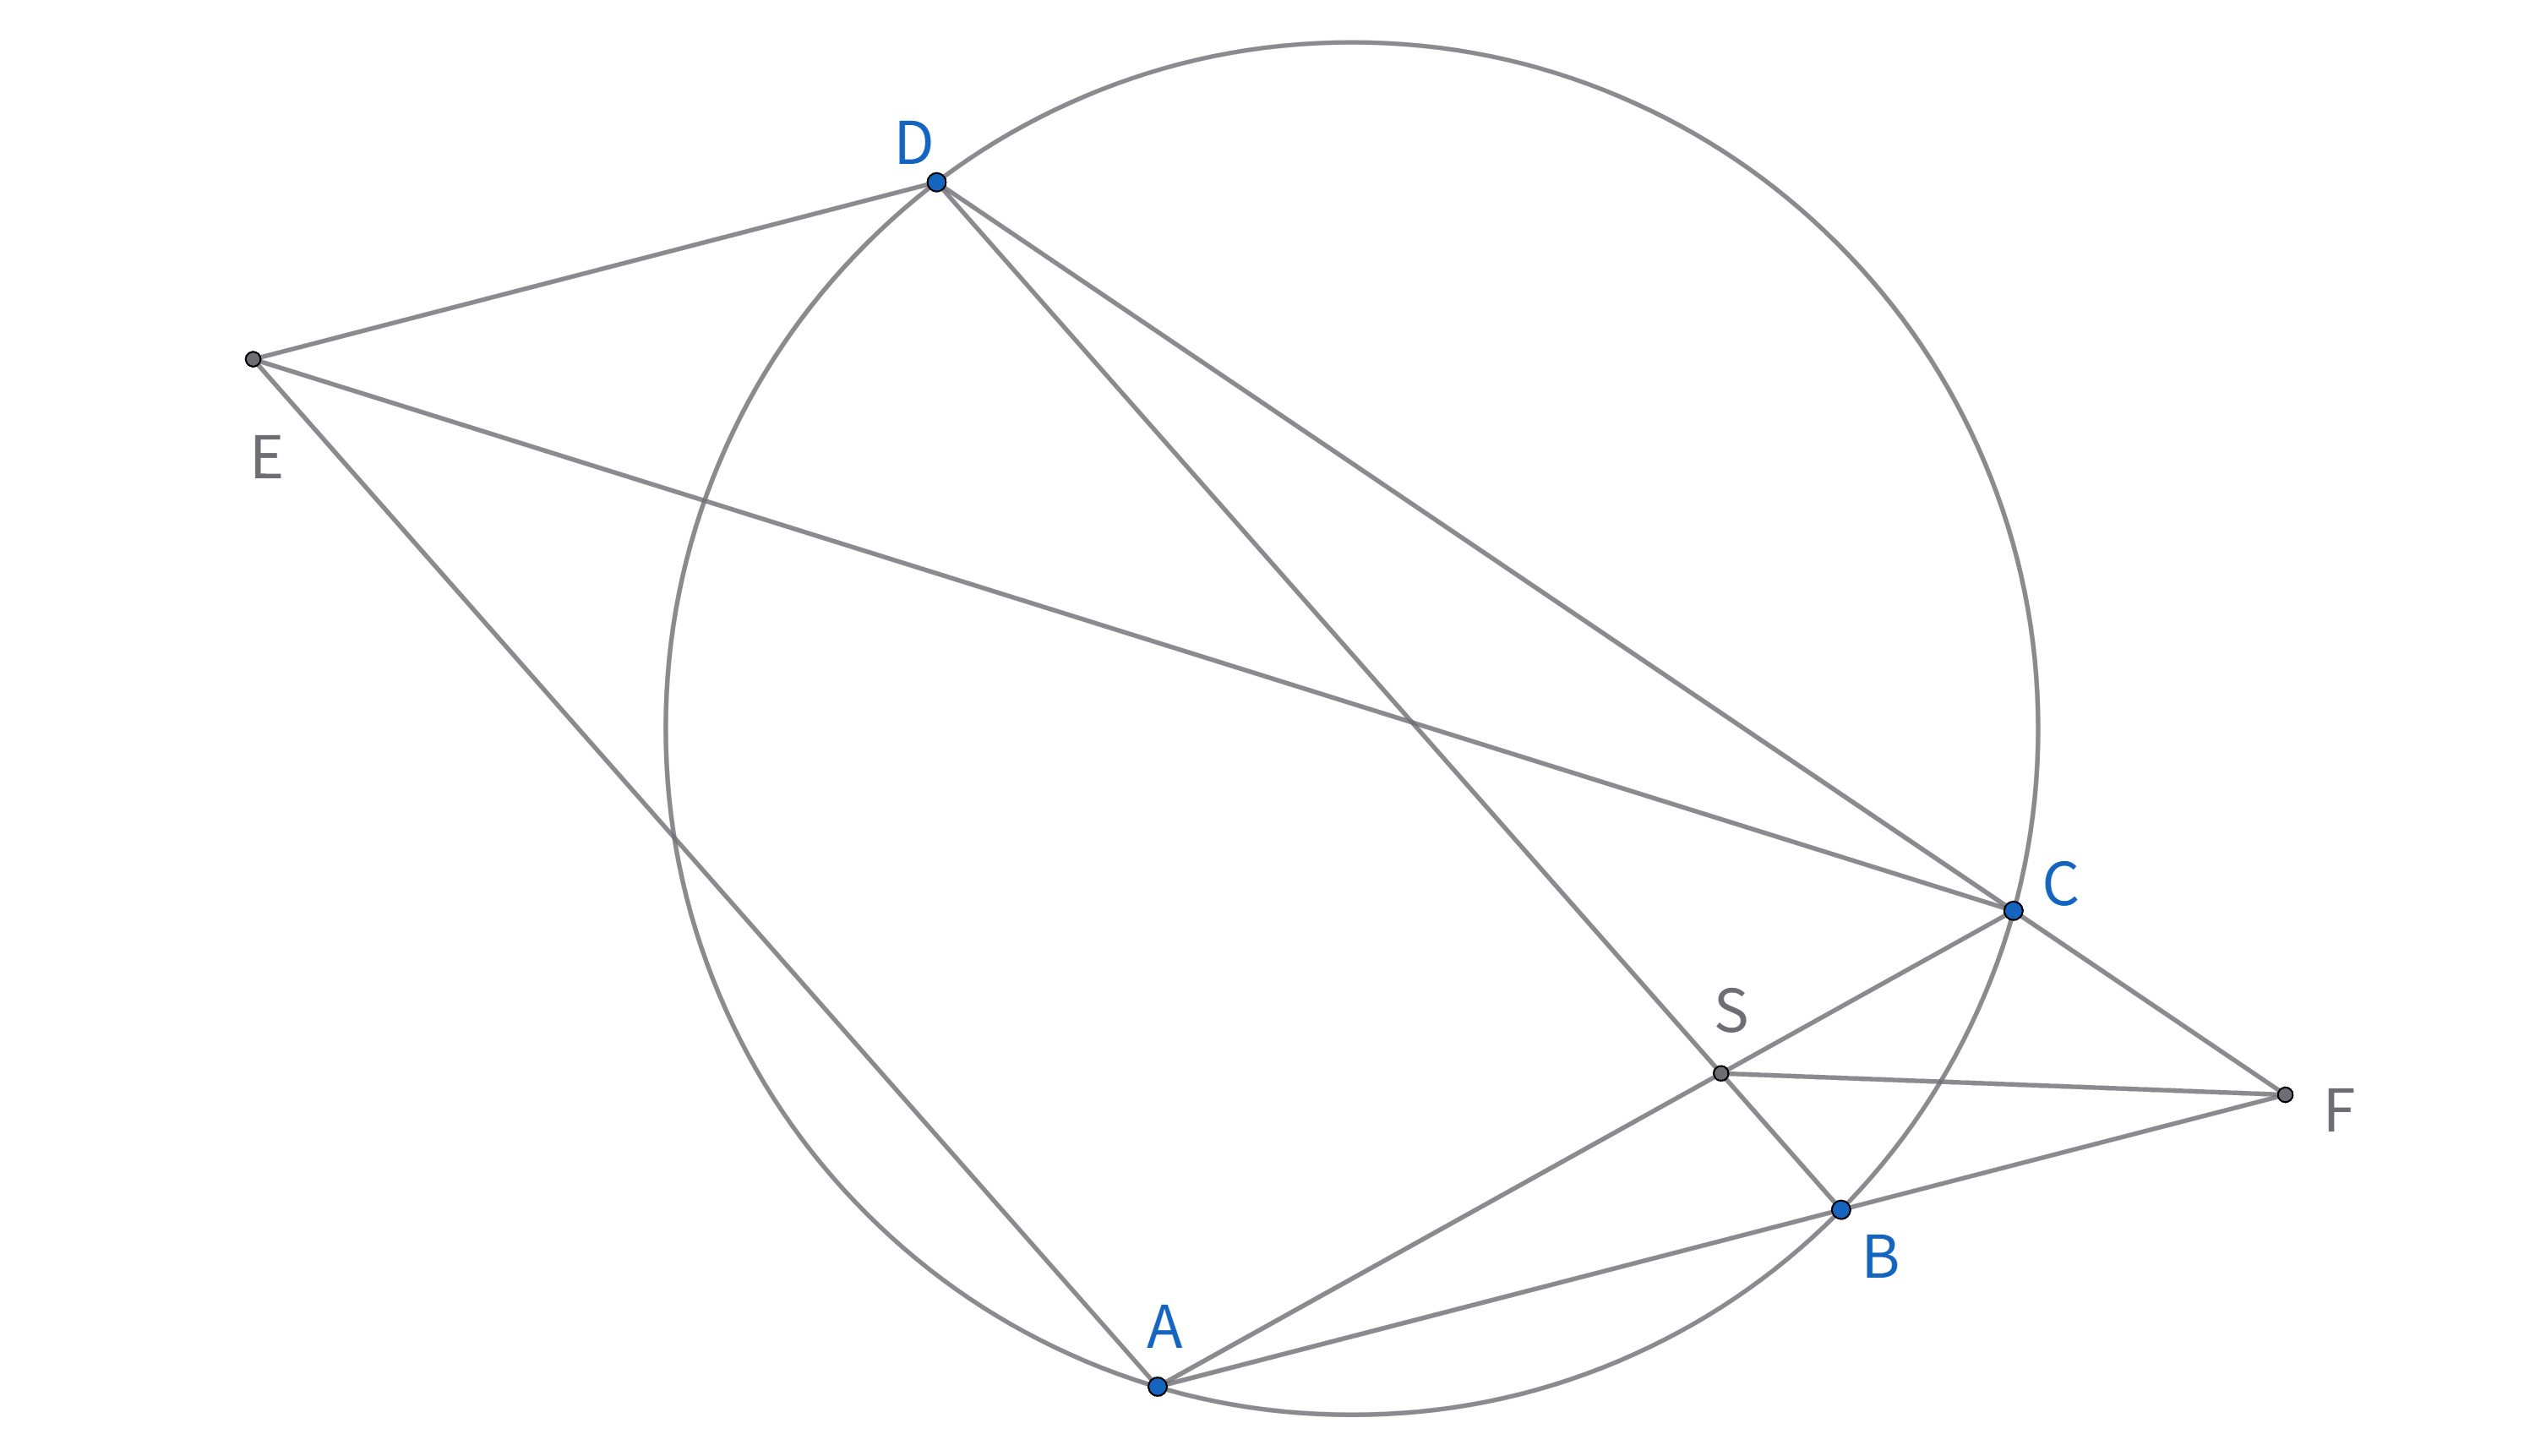
\includegraphics[width=0.9\linewidth]{figures/Q1.png}
\end{figure}


%-------------------------------------------------------------
\newpage 
\subsection{Q2}
已知$\triangle ABF, \triangle AGC$是等边三角形,AD平行于FG。
证明:$CD\parallel BF.$
\begin{figure}[htbp]
    \centering
    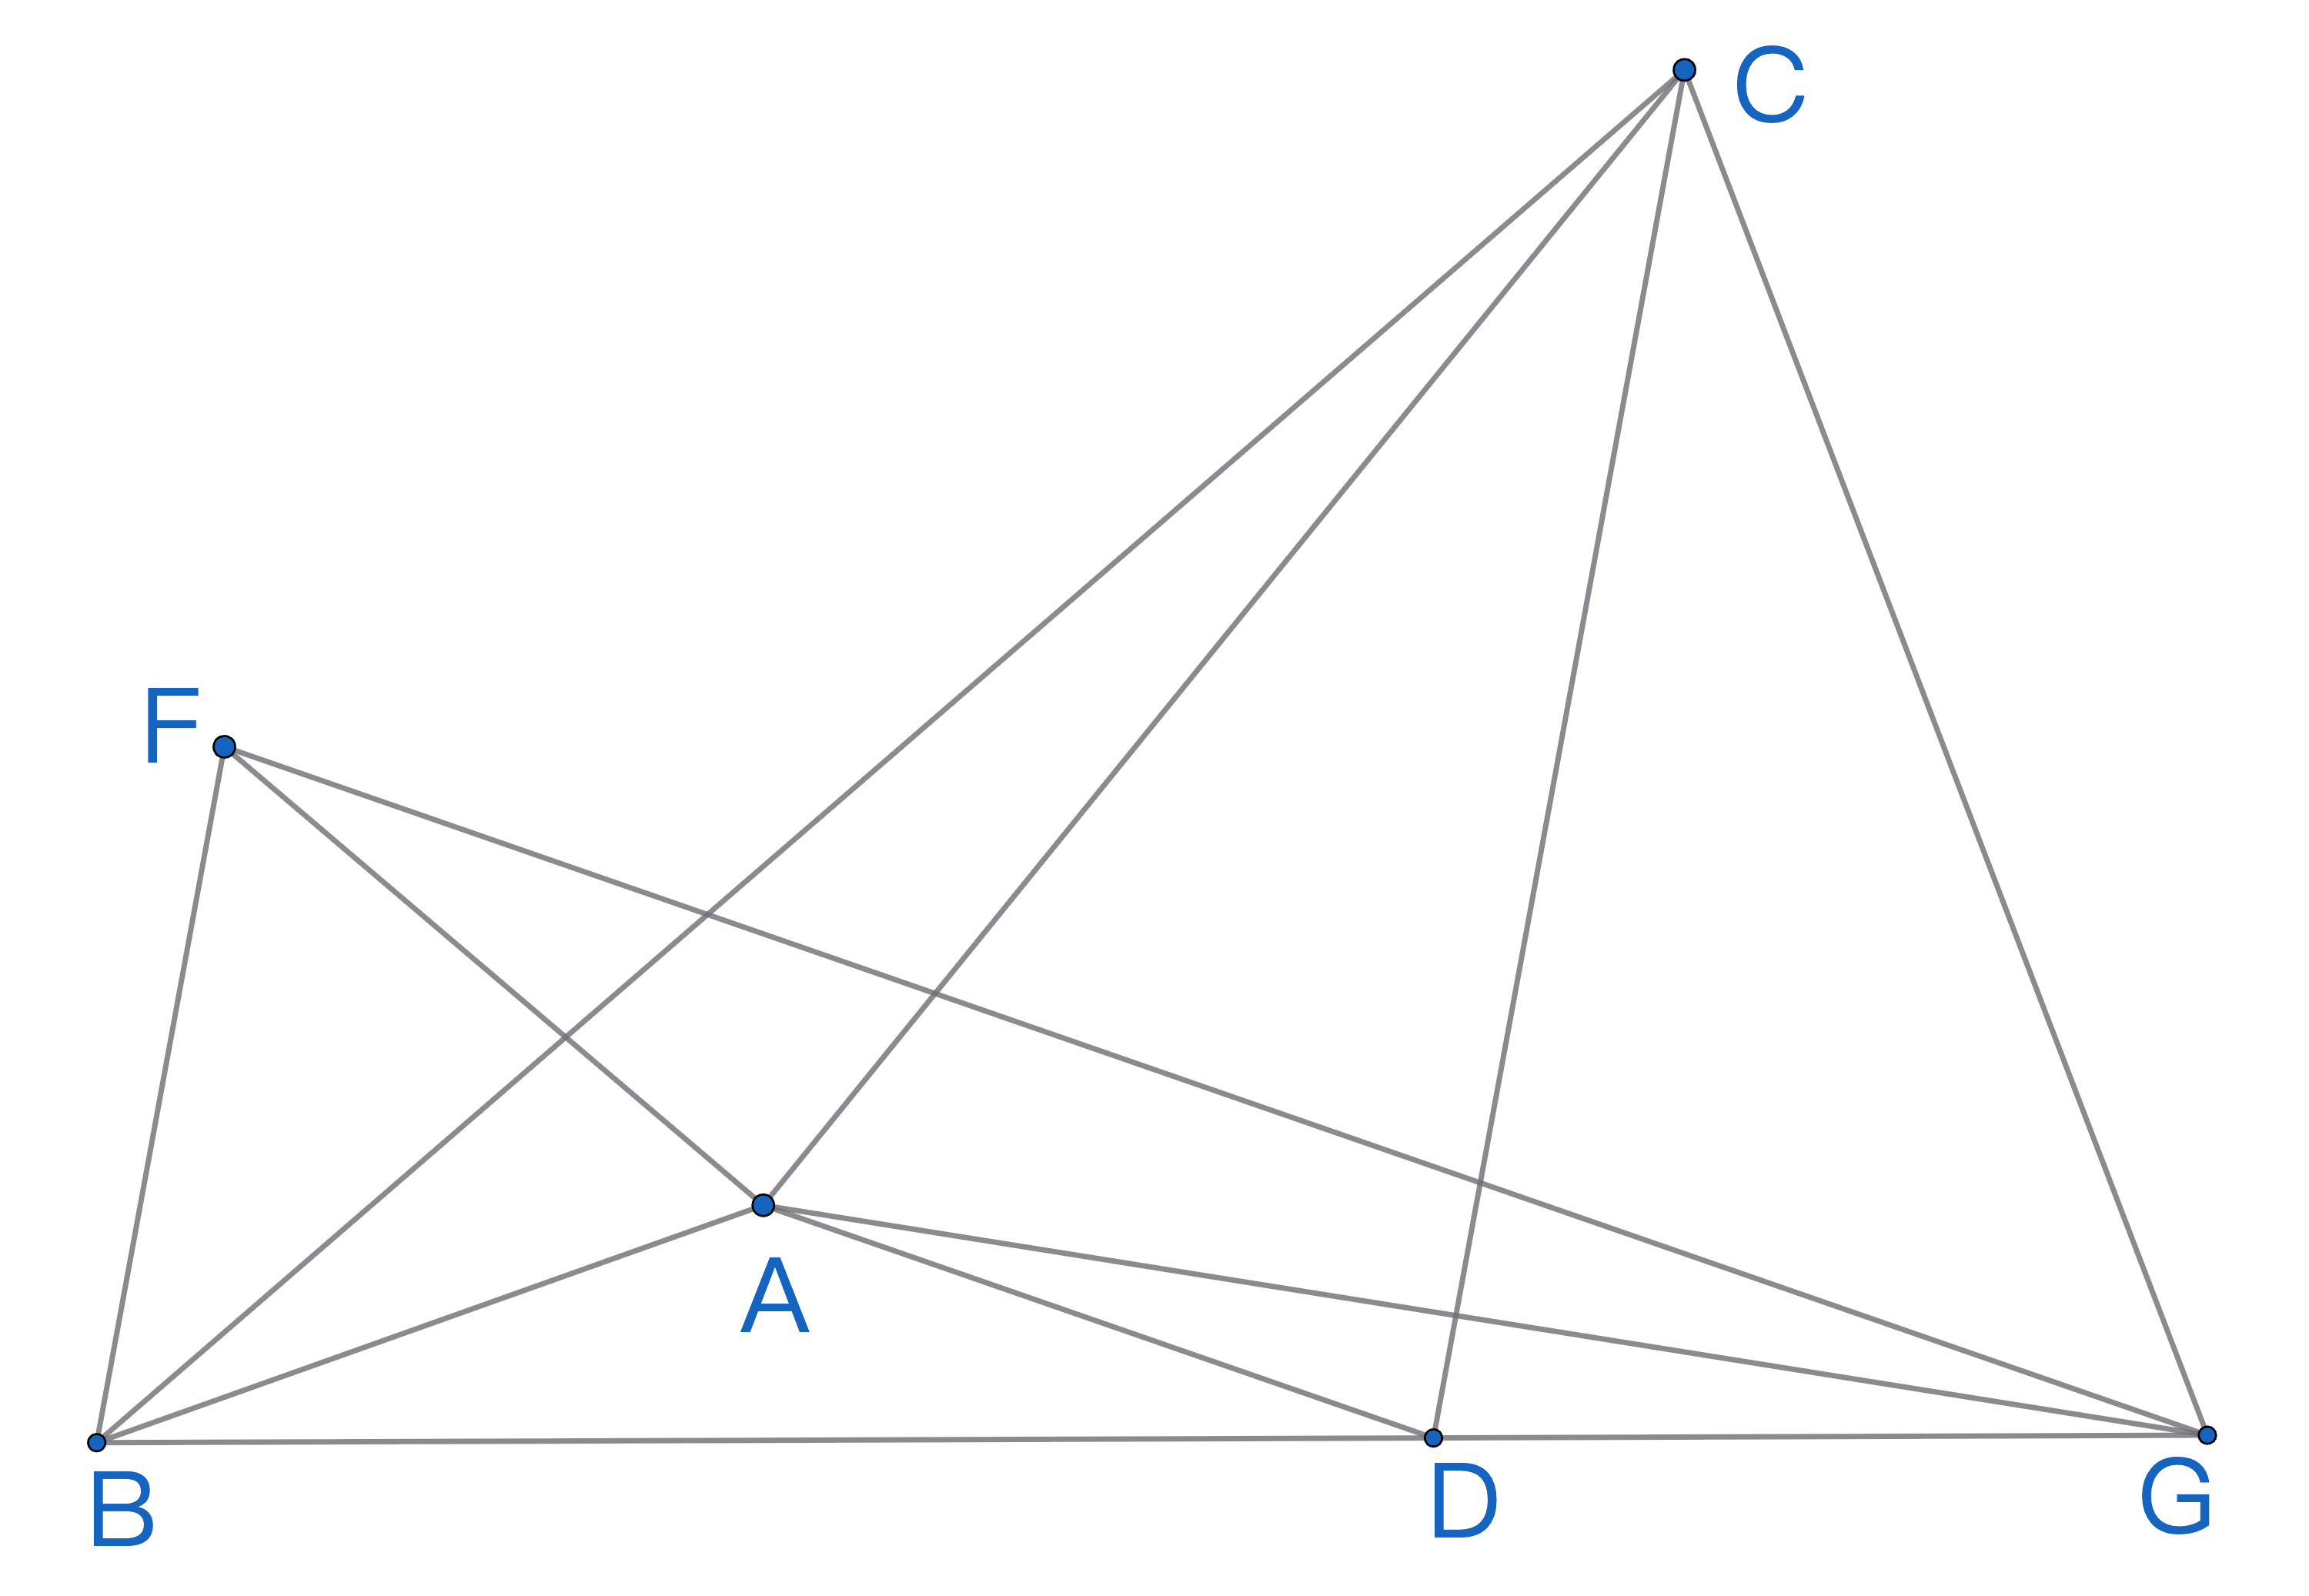
\includegraphics[width=0.7\linewidth]{figures/Q2.png}
\end{figure}


\subsection{Q3}
已知O、I是$\triangle ABC$外心、内心,CI、BI分别交AB、AC于E、F,
$\angle BAC$角平分线交$\triangle ABC$外接圆O于D,M是OI中点。
证明:$DM \perp EF.$
\begin{figure}[htbp]
    \centering
    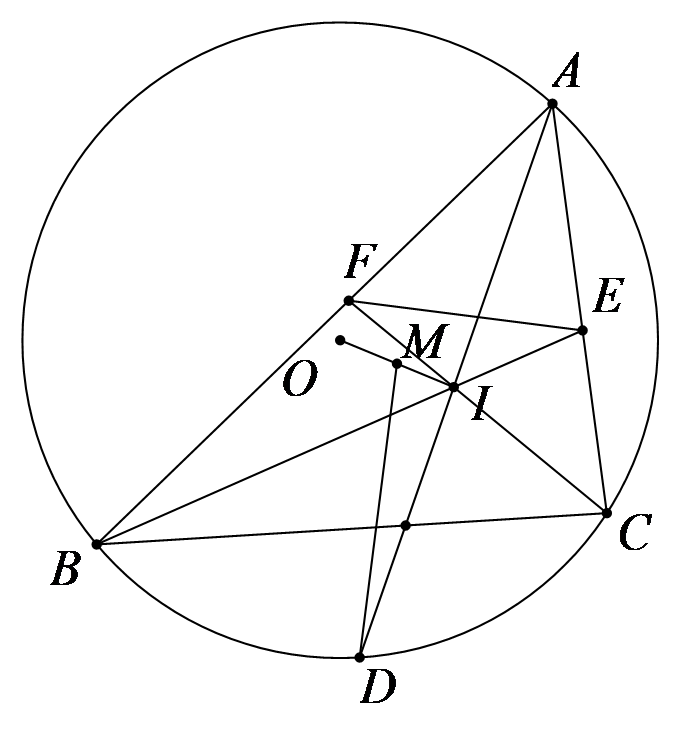
\includegraphics[width=0.6\linewidth]{figures/Q3.png}
\end{figure}



%-------------------------------------------------------------
\newpage 
\subsection{Q4}
已知O、H是$\triangle ABC$的外心、垂心,XY是$\triangle ABC$外接圆O的弦,且XY平行于BC,YH延长线交圆O于D,过D作AX垂线,交圆O于E,XE交BC于J。
证明:$OJ\parallel AX.$
\begin{figure}[htbp]
    \centering
    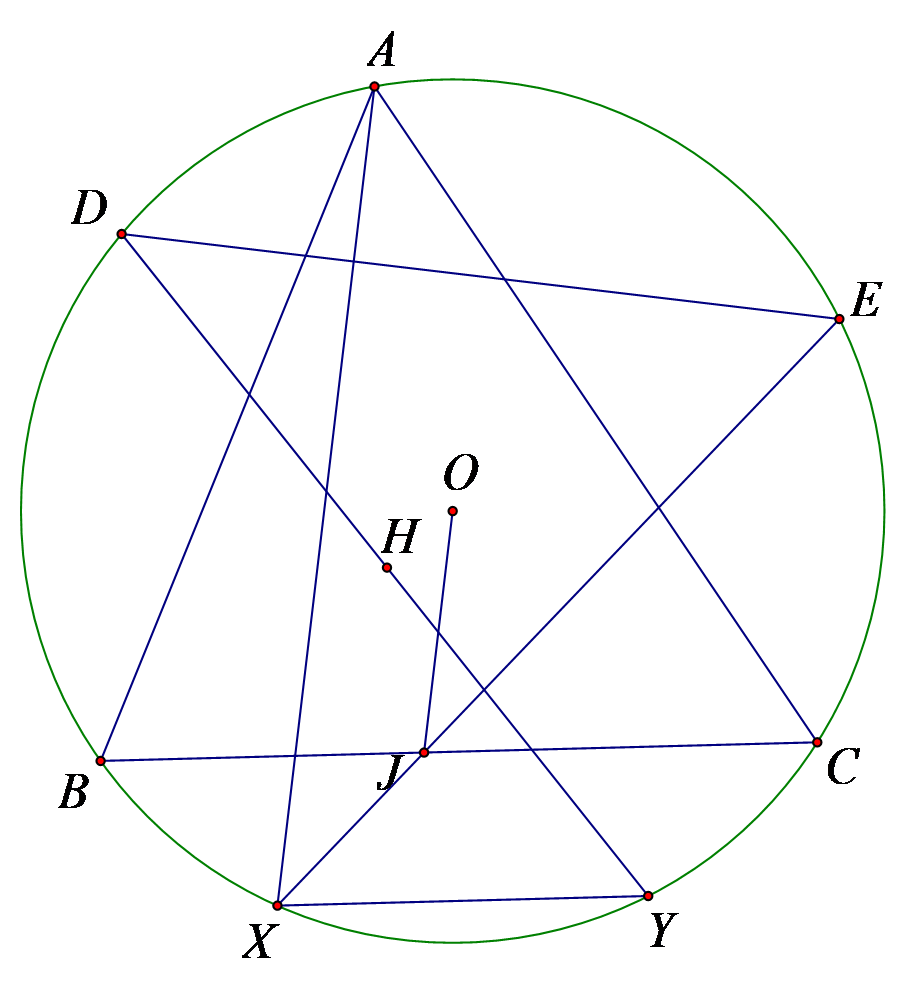
\includegraphics[width=0.4\linewidth]{figures/Q4.png}
\end{figure}

\subsection{Q5}
已知$\triangle ABC$中AH为BC边上的高线,PB、PC是$\triangle ABC$外接圆切线,F在BC上满足$CH=BF$,过F做PF垂线交AB于J,交AC于G。
证明:$\angle GPC=\angle BPJ.$
\begin{figure}[htbp]
    \centering
    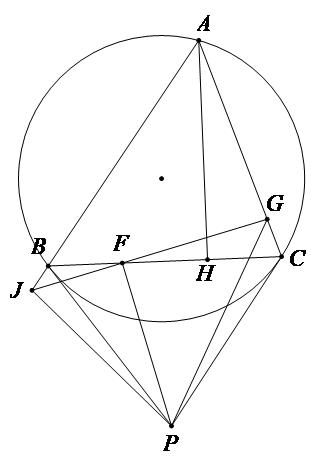
\includegraphics[width=0.4\linewidth]{figures/Q5.png}
\end{figure}

%-------------------------------------------------------------
\newpage
\subsection{Q6}
已知 $AD$ 是 $\angle BAC$ 的角平分线,$T$ 是 $AD$ 上一点,$BT$、$CT$ 分别交 $\triangle ABC$ 的外接圆 $\odot O$ 于 $E$、$F$,$FD$、$ED$ 分别交 $\odot O$ 于 $Y$、$X$,$FX$ 与 $AB$ 交于 $M$,$EY$ 与 $AC$ 交于 $N$。
证明:$MN \parallel BC$
\begin{figure}[htbp]
    \centering
    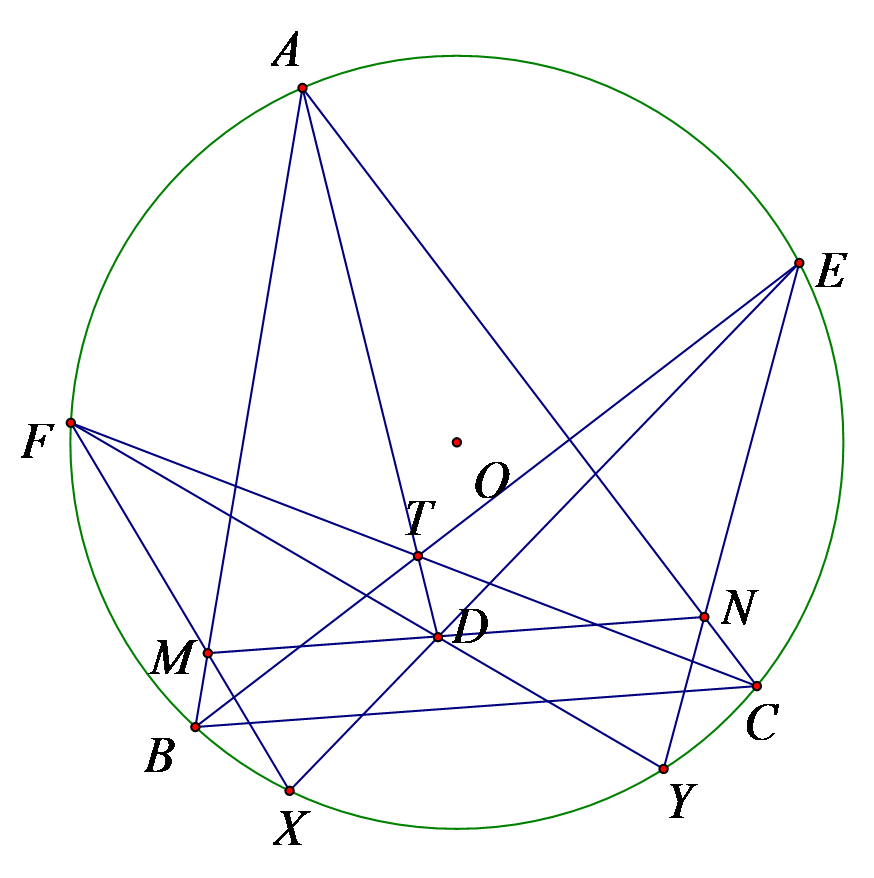
\includegraphics[width=0.5\linewidth]{figures/Q6.png}
\end{figure}

\subsection{Q7}
已知圆 $O_1$,圆 $O_2$ 分别是 $\triangle ABC$ 伪旁切圆,在 $AB$,$AC$ 上切点分别是 $F$,$E$,过 $O_1$,$O_2$ 作 $AC$,$AB$ 垂线交于点 $P$。
证明:$AP \perp EF.$
\begin{figure}[htbp]
    \centering
    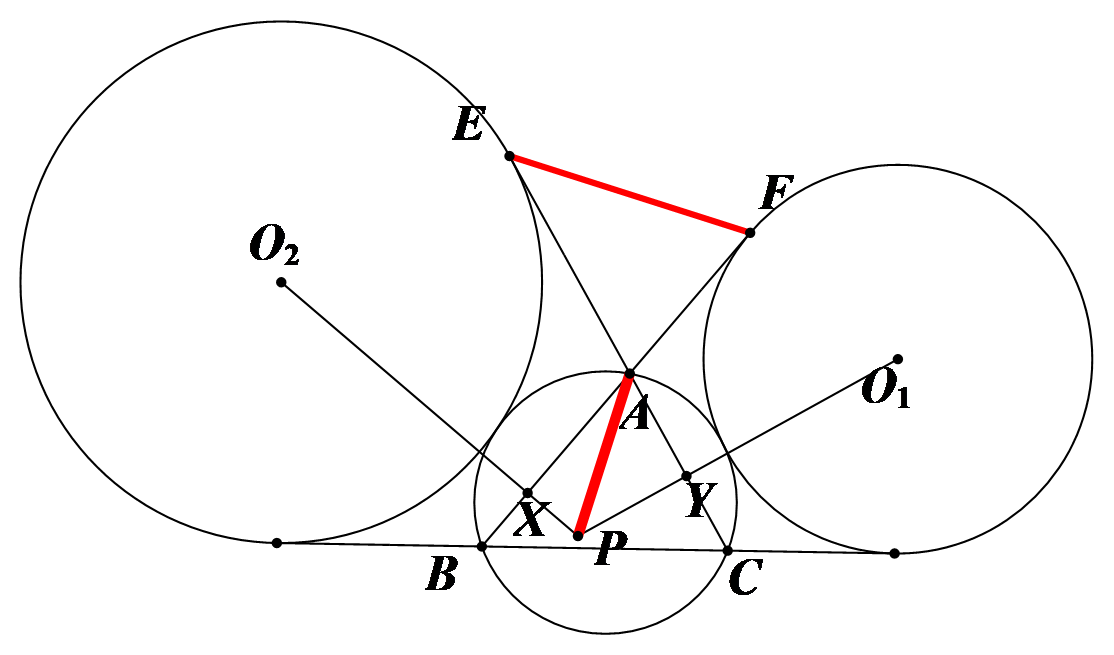
\includegraphics[width=0.8\linewidth]{figures/Q7.png}
\end{figure}

%-------------------------------------------------------------
\newpage
\subsection{Q8}
已知 点 $I$ 是 $\triangle ABC$ 内心,直线 $BI$、$CI$ 交 $AC$、$AB$ 分别于 $E$、$F$,点 $I'$、$I$ 关于 $BC$ 对称,$ID' \perp BE$,$I'G \perp CF$,分别交 $BC$ 于 $D$、$G$。
求证 $\angle BGF = \angle CDE.$
\begin{figure}[htbp]
    \centering
    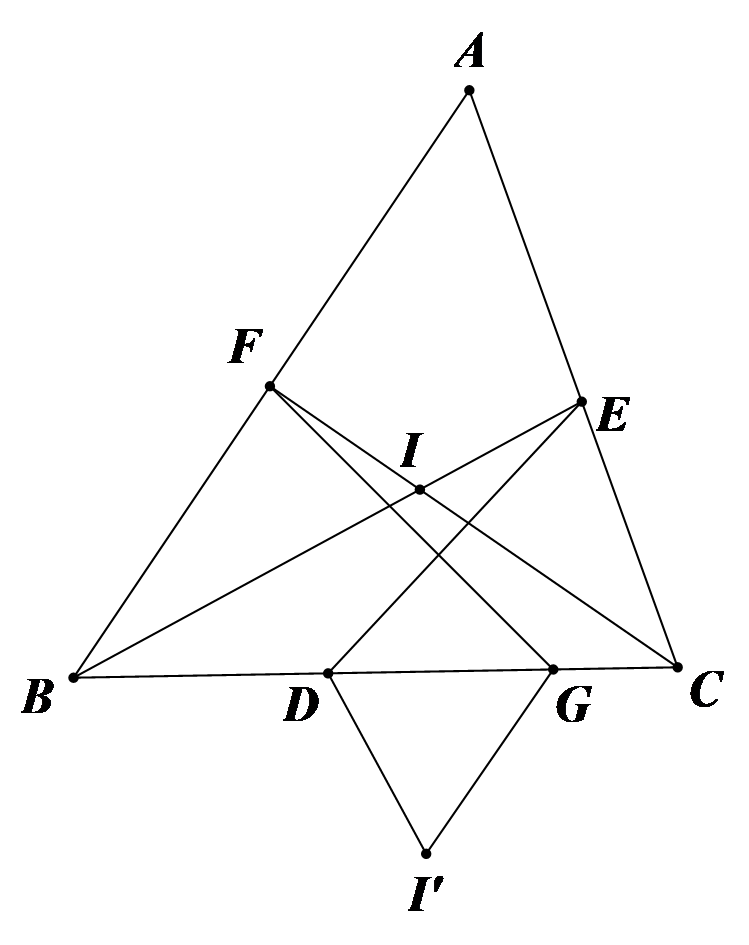
\includegraphics[width=0.5\linewidth]{figures/Q8.png}
\end{figure}

\subsection{Q9}
已知 $H$、$O$ 是 $\triangle ABC$ 垂心,外心,$D$ 是 $BC$ 中点,过 $H$ 作$BC$ 平行线交 $AD$ 于 $G$,$AO$ 交 $BH$ 于 $E$。
求证:$GH = EG.$
\begin{figure}[htbp]
    \centering
    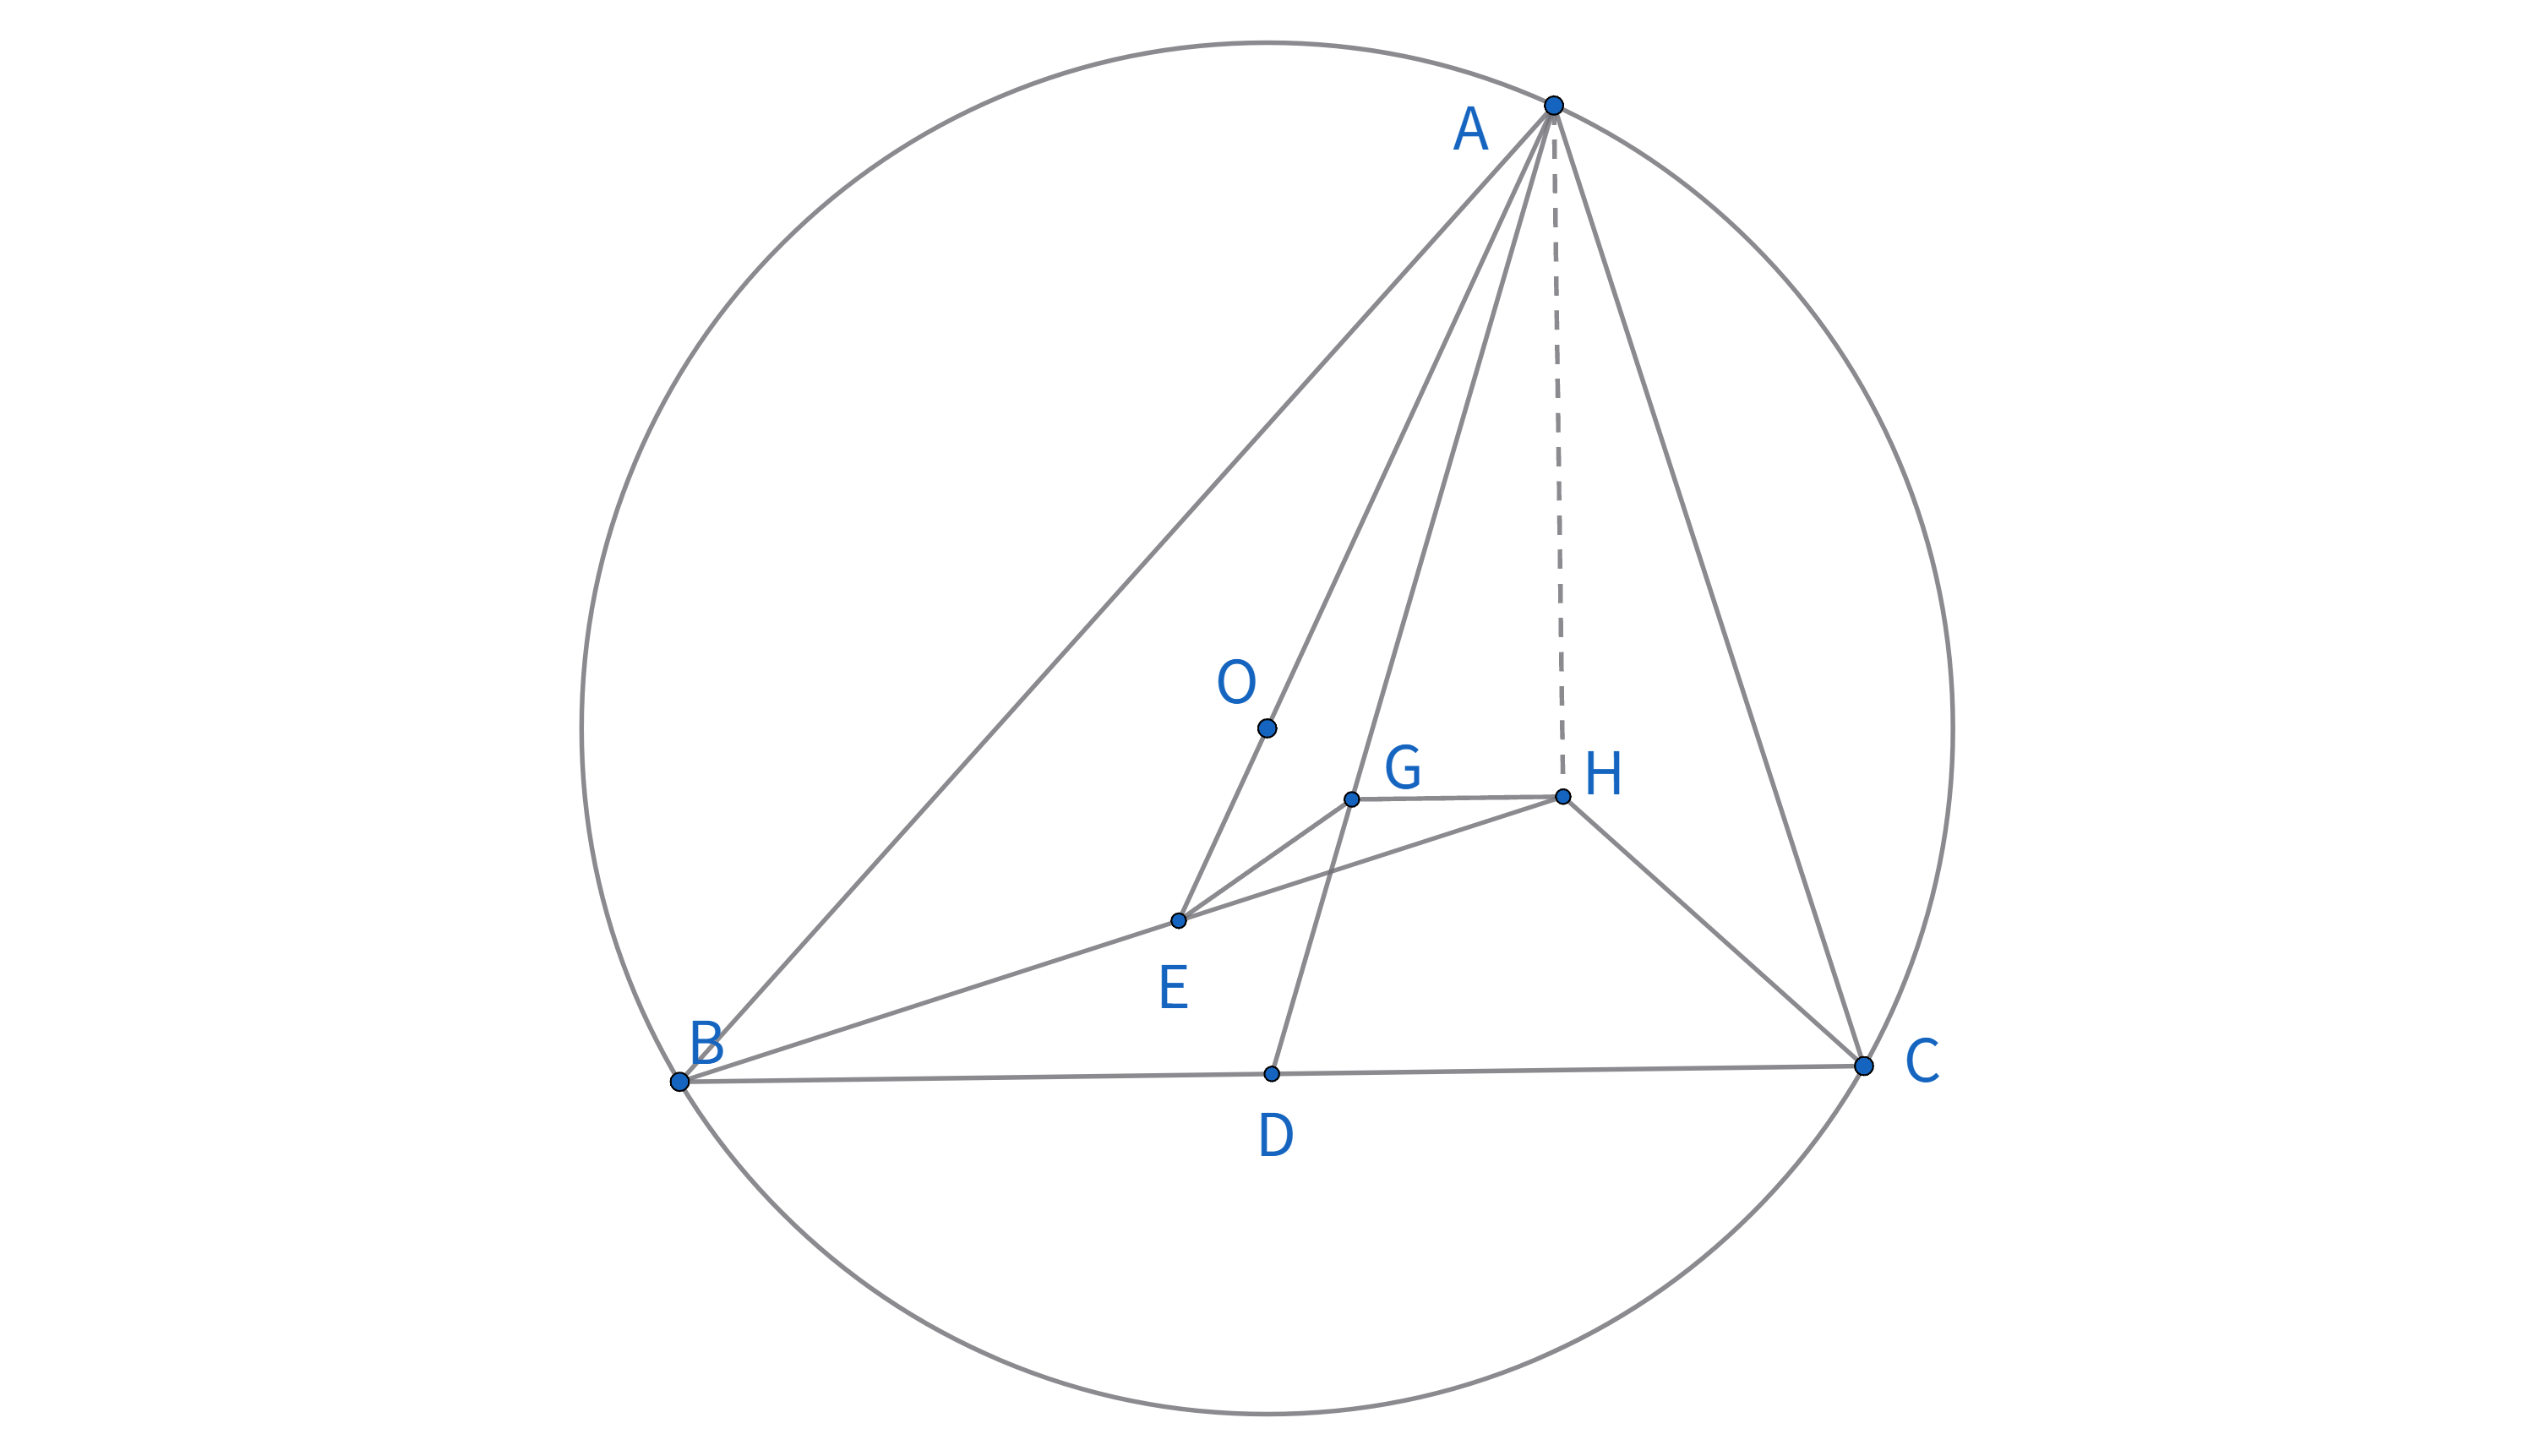
\includegraphics[width=0.9\linewidth]{figures/Q9.png}
\end{figure}
%-------------------------------------------------------------
\newpage
\subsection{Q10}
$\triangle ABC$ 内接于圆 $O$,$H$ 为垂心,过 $A$ 作 $OH$ 垂线交外接圆于 $P$,$OH$ 交 $BC$ 延长线于 $K$,连接 $AK$ 交外接圆于 $Q$,取 $T$ 使得 $ACTB$ 为平行四边形。证明:$T$、$P$、$H$、$Q$ 四点共圆。
\begin{figure}[htbp]
    \centering
    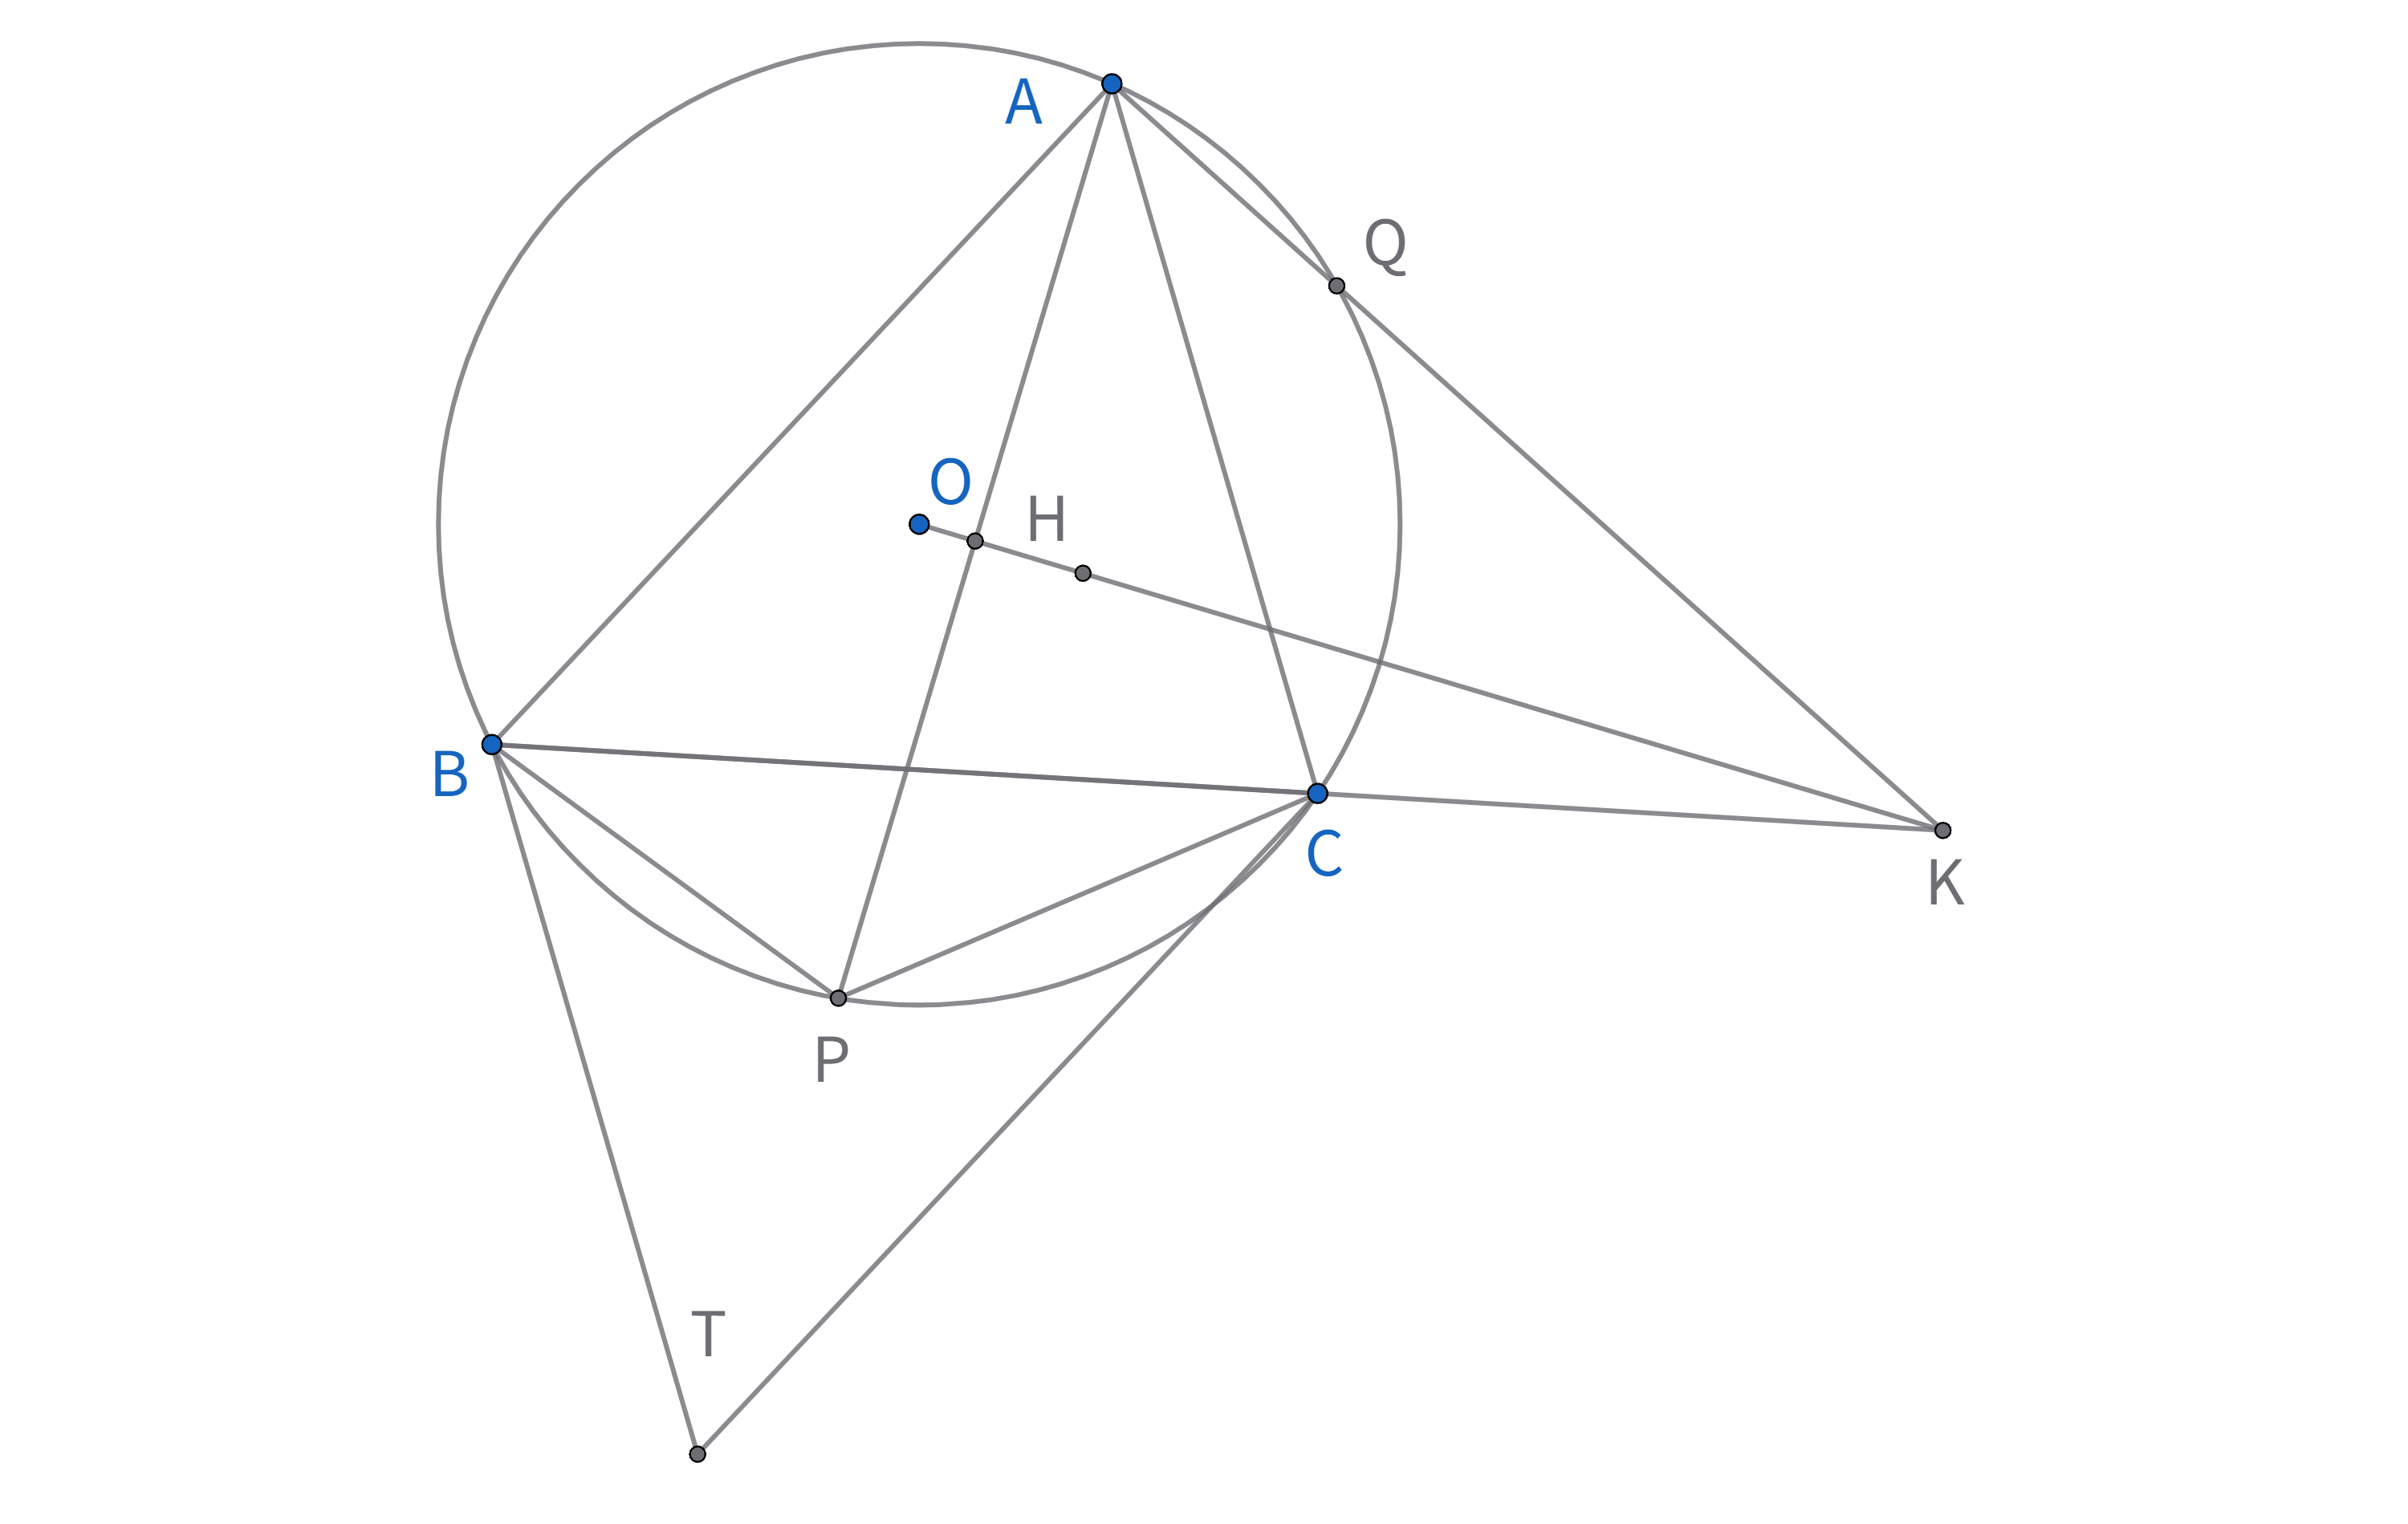
\includegraphics[width=0.9\linewidth]{figures/Q10.png}
\end{figure}

\subsection{Q11}
在 $\triangle ABC$ 中,$H$ 是垂心,$BE$、$CF$ 是高,$\angle BAC$ 的角平分线交 $EF$ 于 $X$,$\angle EHF$ 的角平分线交 $EF$ 于 $Y$,$EF$ 交 $\triangle AXH$ 的外接圆于 $P$,交 $\triangle AYH$ 的外接圆于 $Q$。
证明:$B$、$C$、$Q$、$P$ 四点共圆。
\begin{figure}[htbp]
    \centering
    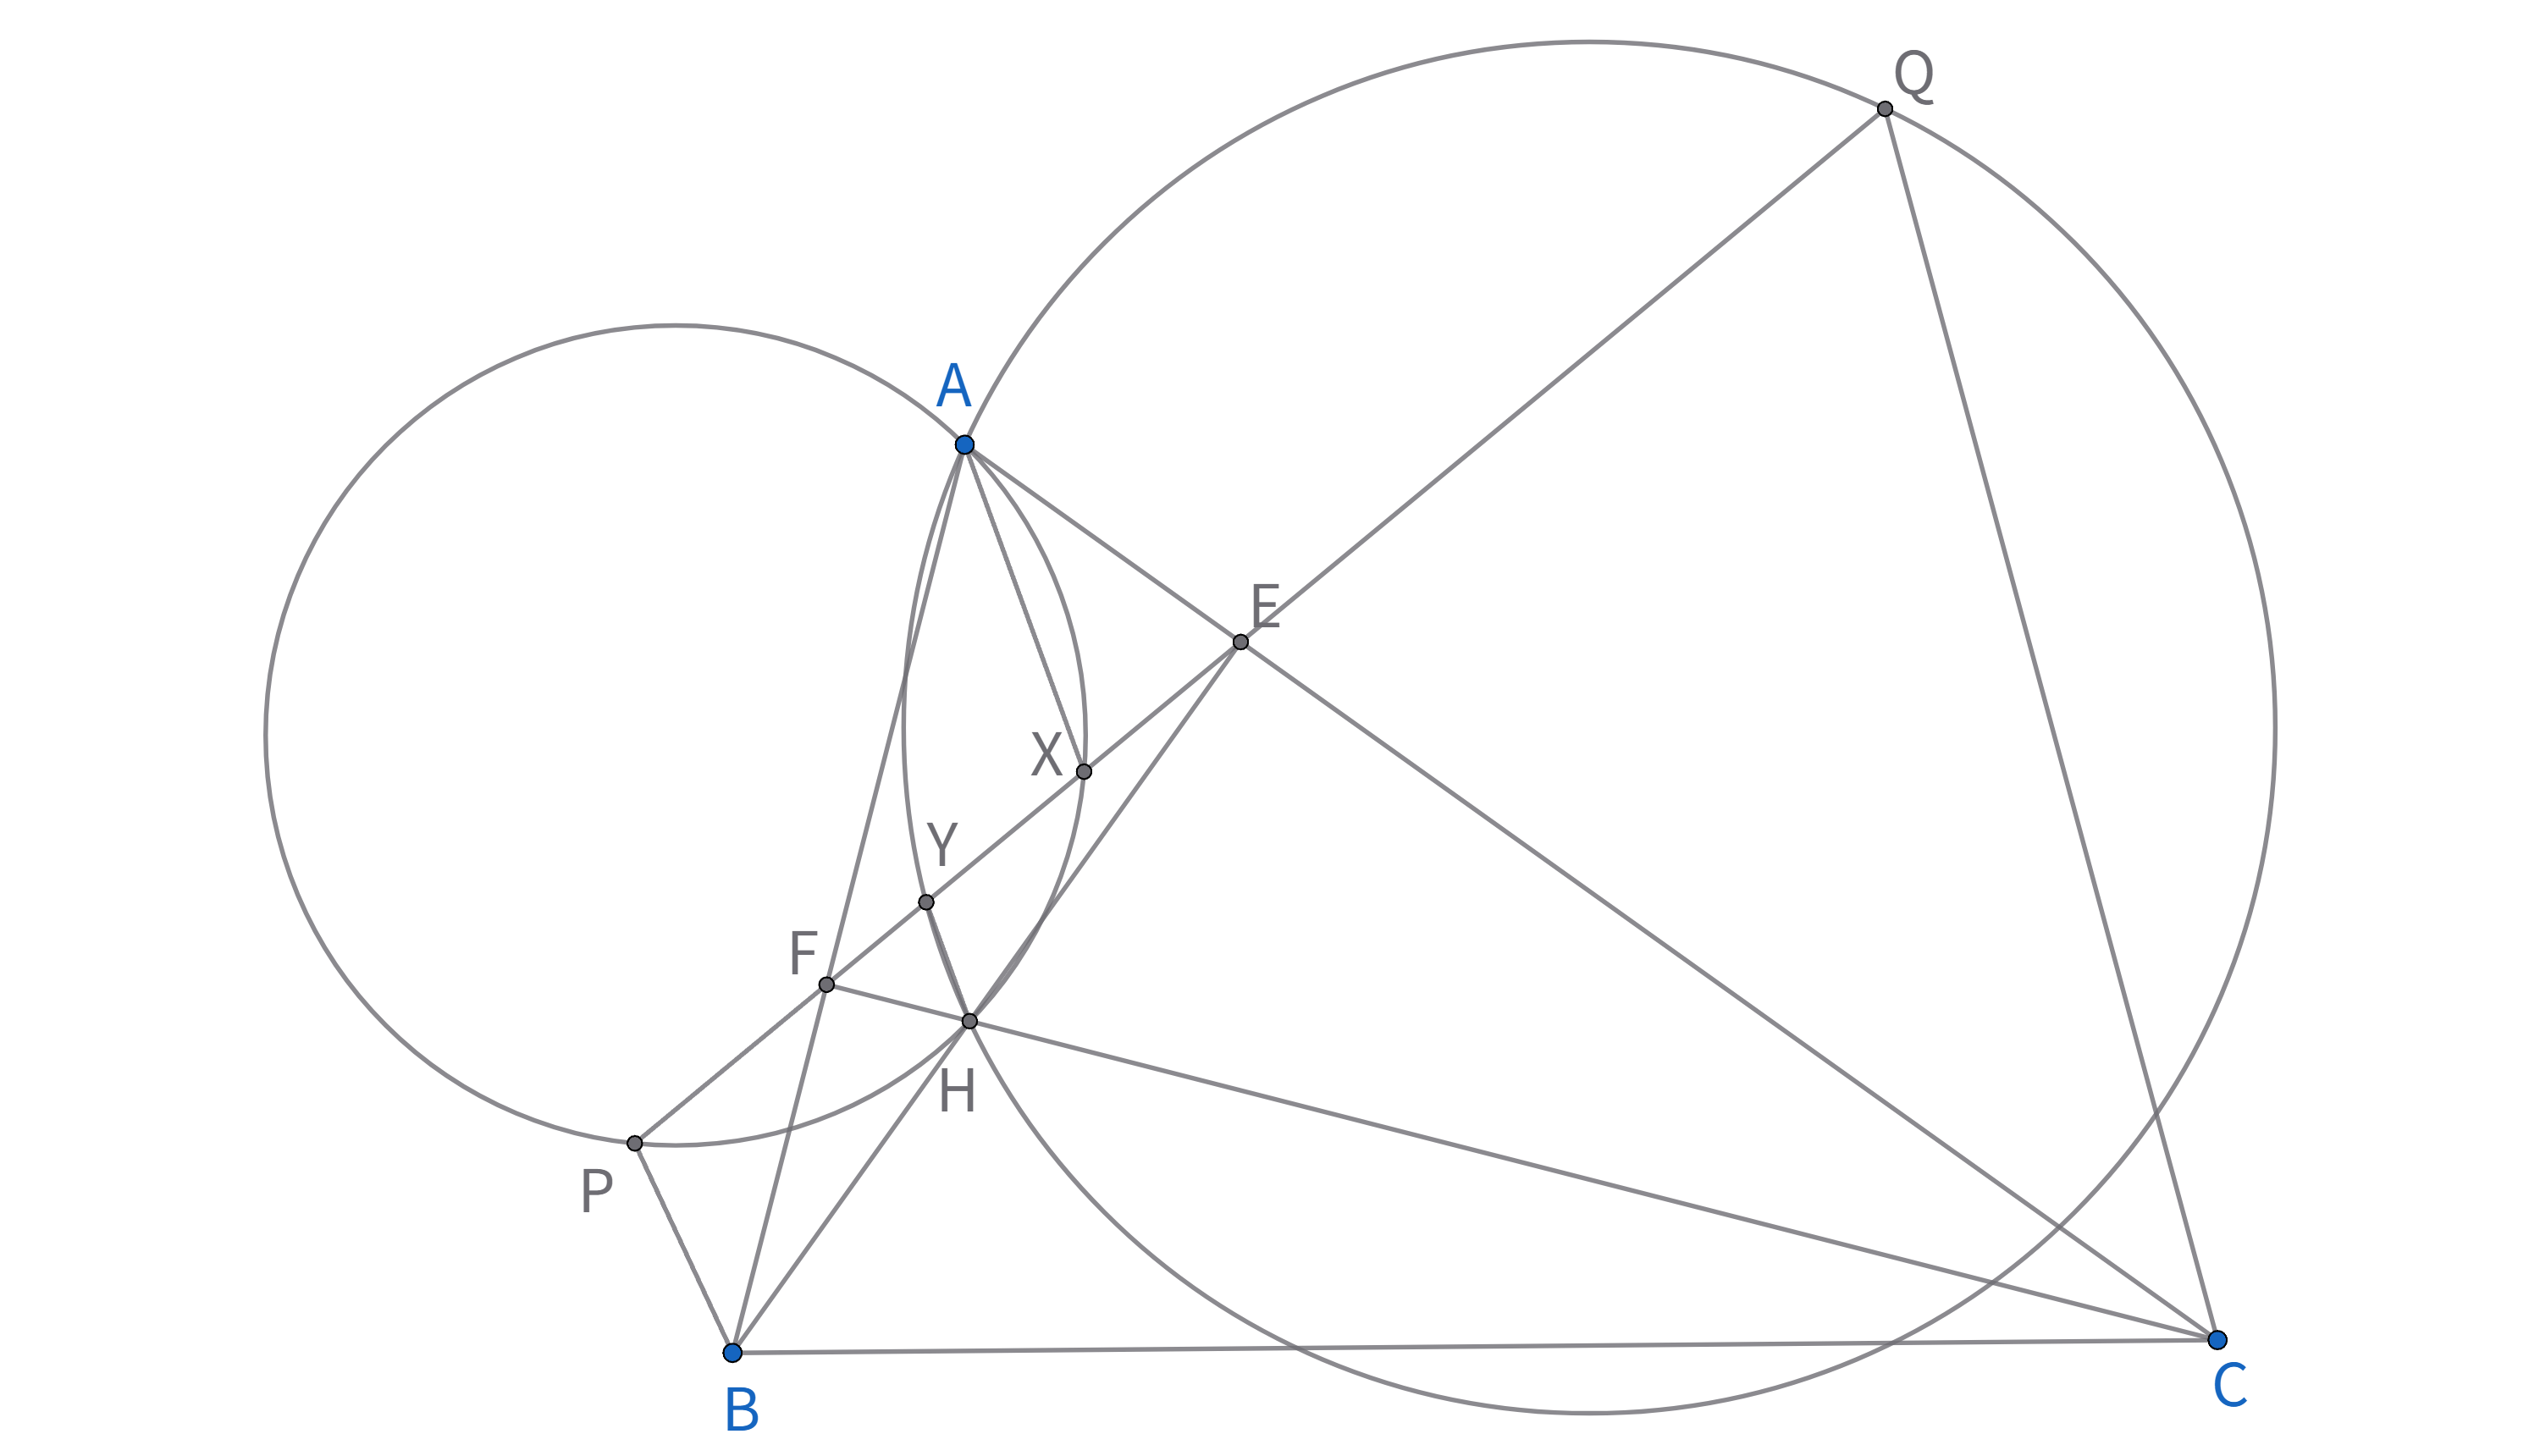
\includegraphics[width=0.9\linewidth]{figures/Q11.png}
\end{figure}

\end{document}